\documentclass{article}
\usepackage{arxiv}

\usepackage[utf8]{inputenc}
\usepackage[english, russian]{babel}
\usepackage[T1]{fontenc}
\usepackage{url}
\usepackage{booktabs}
\usepackage{amsfonts}
\usepackage{nicefrac}
\usepackage{microtype}
\usepackage{graphicx}
\usepackage{natbib}
\usepackage{doi}
\usepackage{cmap}

\usepackage{svg}
\usepackage{caption}
\usepackage{subcaption}
\usepackage{ucs}
\usepackage{gensymb}

\usepackage{algorithm}
\usepackage{algpseudocode}
\usepackage{amssymb, amsmath, mathrsfs, amsthm}
\usepackage{bbm}
\usepackage{bm}
\usepackage{color}
\usepackage{csvsimple}
\usepackage{fancyvrb}
\usepackage{graphicx}
\usepackage[hidelinks]{hyperref}
\usepackage{indentfirst}
\usepackage{listings}
\usepackage{mathtools}
\usepackage{multirow}
\usepackage{pgfplots}
\pgfplotsset{compat=1.18}

\usepackage{tikz}
\usepackage{wrapfig}
\usepackage{yfonts}



\title{Использование пространственно-временных зависимостей для мониторинга аддитивного производства с применением глубокого обучения}

\author{Vladislav Soldatov\\
	\texttt{worklikewalkietalkie@gmail.com} \\
	%% examples of more authors
	\And
	  Dmitry Kropotov \\
	\texttt{dmitry.kropotov@gmail.com} \\
	%% \AND
	%% Coauthor \\
	%% Affiliation \\
	%% Address \\
	%% \texttt{email} \\
	%% \And
	%% Coauthor \\
	%% Affiliation \\
	%% Address \\
	%% \texttt{email} \\
	%% \And
	%% Coauthor \\
	%% Affiliation \\
	%% Address \\
	%% \texttt{email} \\
}
\date{}

\renewcommand{\shorttitle}{\textit{arXiv} Template}

%%% Add PDF metadata to help others organize their library
%%% Once the PDF is generated, you can check the metadata with
%%% $ pdfinfo template.pdf
\hypersetup{
pdftitle={Использование пространственно-временных зависимостей для мониторинга аддитивного производства с применением глубокого обучения},
pdfsubject={q-bio.NC, q-bio.QM},
pdfauthor={Vladislav Soldatov, Dmitry Kropotov},
pdfkeywords={Additive manufacturing, Laser Powder Bed Fusion, Online
monitoring, Flaw detection, Porosity prediction, Spatial-temporal Modeling},
}

\begin{document}
\maketitle

\begin{abstract}
	Мониторинг процессов аддитивного производства в режиме реального времени необходим для обеспечения качества деталей и предотвращения дефектов, так как лазерное сплавление в порошковом слое -- это динамический и сложный процесс. Однако существующие алгоритмы мониторинга в режиме реального времени часто зависят от конкретного случая и не устойчивы к изменениям параметров процесса или типов данных. В данной работе рассмотрен один из методов глубокого обучения, ранее использованных для решения этой проблемы, а также предложен новый подход к задаче. Кроме того, было проведено исследование вышеупомянутых алгоритмов и их сравнение на наборе данных NIST <<Overhang Part X4>>. 
\end{abstract}


\keywords{Additive manufacturing $\cdot{}$ Laser Powder Bed Fusion $\cdot{}$ Online monitoring $\cdot{}$ Flaw detection $\cdot{}$ Porosity prediction $\cdot{}$ Spatial-temporal Modeling}

\section{Введение}
    Аддитивное производство (АП) - это быстро развивающаяся технология, которая потенциально способна произвести революцию в обрабатывающей промышленности~\cite{AMisCool}. Технология АП позволяет создавать сложные, легкие и высокопроизводительные детали, которые было бы трудно или невозможно изготовить традиционными методами. Однако процессы АП сложны и могут быть подвержены дефектам. Использование аддитивного производства в промышленности в настоящее время ограничено из-за неизвестного заранее и ненадежного качества деталей~\cite{Grasso2017ProcessDA}. Это в значительной степени вызвано сложными взаимосвязями между параметрами процесса, такими как мощность лазера, скорость лазерного излучения и другими настройками машины. Поэтому важно разработать методы мониторинга процессов АП в режиме реального времени для обеспечения качества деталей.

    Несмотря на возможность использования статистических~\cite{gaussian_process} методов и классических алгоритмов машинного обучения~\cite{classic_ml}, одним из многообещающих подходов к мониторингу процессов АП в режиме реального времени является использование глубокого обучения (DL). В данной работе представлен новый подход к использованию DL для мониторинга процессов АП в режиме реального времени и проведено сравнение с одним из лучших алгоритмов для данной задачи на настоящий момент, ConvLSTMAE~\cite{convlstm_nist}. Как предлагаемый, так и существующий подходы используют пространственно-временную модель для изучения взаимосвязей между параметрами процесса и качеством детали. Пространственно-временная модель учитывает динамическую природу процессов АП. Это позволяет рассматриваемым подходам быть более точными, чем традиционные методы, которые учитывают только статические зависимости между параметрами процесса и качеством детали.

\section{Обзор задачи}
    Процессы АП сильно варьируются в зависимости от таких факторов, как свойства используемых материалов, качество платформы для сборки и квалификация оператора. Эта изменчивость затрудняет разработку моделей, которые могут точно предсказать поведение процессов АП при любых условиях. Например, свойства используемых материалов могут влиять на температуру плавления металла, которую необходимо учитывать при построении алгоритма, использующего физические признаки управляемого процесса.

    Помимо этого, процессы АП очень динамичны и включают в себя множество взаимодействующих факторов. Например, всплески ванны лазерного расплава могут влиять на поток расплавленного металла, что, в свою очередь, может повлиять на форму и пористость изготавливаемой детали.

    Таким образом, основная сложность исследований в сфере мониторинга процессов АП заключается в том, что существует большое количество разнообразных установок, отличающихся производственными возможностями, настройками и параметрами. В связи с этим довольно трудоёмким оказывается процесс стандартизации и обобщения условий, в которых метод мониторинга АП должен осуществлять работу. В результате, создание универсальной модели, которую можно было бы использовать для мониторинга всех машин АП, становится затруднено.
    
    Другой проблемой является нехватка наборов данных, на основе которых можно обучать и тестировать модели DL. Наборы данных для мониторинга процессов АП обычно собираются с использованием систем с замкнутым контуром~\cite{closed-loop}. Системы с замкнутым контуром контролируют процесс АП в режиме реального времени и используют эту информацию для настройки параметров процесса. Это затрудняет сбор наборов данных, репрезентативных для всего спектра возможных условий процесса АП. Кроме того, организации, занимающиеся подобными исследованиями, проводят их на наборах закрытых данных для внутреннего пользования, собранных на конкретной установке, доступной соответствующей организации.

    В данной работе основной фокус внимания был уделён направлению АП под названием <<Лазерное сплавление в порошковом слое>> (Laser Powder Bed Fusion или LBPF), а в качестве данных использовались изображения лазерных ванн расплава (см. Рис. \ref{meltpool_examples}). Для обучения моделей применялся набор данных <<Overhang Part X4>>~\cite{nist_dataset}. В связи с большим объёмом неразмеченных данных, задача состояла в обучении нейросетей представлениям идущих подряд во времени кадров ванн расплава. Модель должна выдавать в качестве ответа изображение прогнозируемого следующего после входных данных кадра. Это позволяет перейти от постановки задачи в терминах всевозможных используемых материалов и установок АП, к пространству последовательностей кадров ванн расплава, имеющих характерные изменения в форме при проявлении аномалий, идентичные для любых характеристик установок и материалов.

\section{Условия экспериментов}
\subsection{Методология}
    В качестве подхода машинного обучения к задаче в вышеописанной постановке, была выбрана парадигма самообучения (self-supervised learning) на основе автокодировщиков. Модели данного типа могут обнаруживать сложные зависимости в данных, создавая содержательные представления неразмеченных объектов. Процесс создания модели для обнаружения аномальных объектов и последующего её применения состоит из следующих этапов:\begin{enumerate}
        \item Определить и выделить <<нормальные>> (не являющиеся аномальными) объекты выборки.
        \item Обучить автокодировщик на выделенной подвыборке.
        \item По валидационной выборке выбрать порог для значения функционала ошибки восстановления между предсказанным кадром и правильным ответом.
        \item При превышении значения порога на функционал ошибки восстановления, объявлять кадры текущей последовательности аномальными.
    \end{enumerate}
    В качестве функционала ошибки восстановления была выбрана квадратичная ошибка между кадром из выборки и предсказанным кадром: \begin{equation}\label{mse}
        SquaredError(X, \hat{X}) := \sum\limits_{i, j} (X_{ij} - \hat{X}_{ij})^2 = \|X - \hat{X}\|_F^2,
    \end{equation} где $X$ и $\hat{X}$ -- матрицы пиксельных представлений вышеуказанных кадров. 
    

\subsection{Обзор данных}
    В выбранном наборе данных представлены последовательные кадры лазерных ванн расплава, полученные при послойном наплавлении 4 одинаковых деталей, имеющих <<нависания>>, то есть структурные компоненты такие, что на более поздних слоях плавления, новые части детали не имеют под собой опоры в виде уже наплавленного материала. Всего в процессе сбора данных запечатлено 250 последовательных слоёв печати по $20~мкм$. Каждая из 4 деталей имеет размер $5$~мм~$\times~9$~мм~$\times~5$~мм и выплавлена на пластине из кованого никелевого сплава (IN625). Направление плавления меняется на $90\degree$ от слоя к слою. Геометрия деталей на нескольких слоях отображена на Рис. \ref{parts_geom}.

    \begin{figure}[H]
        \center
        \begin{subfigure}{.47\textwidth}
            \centering
            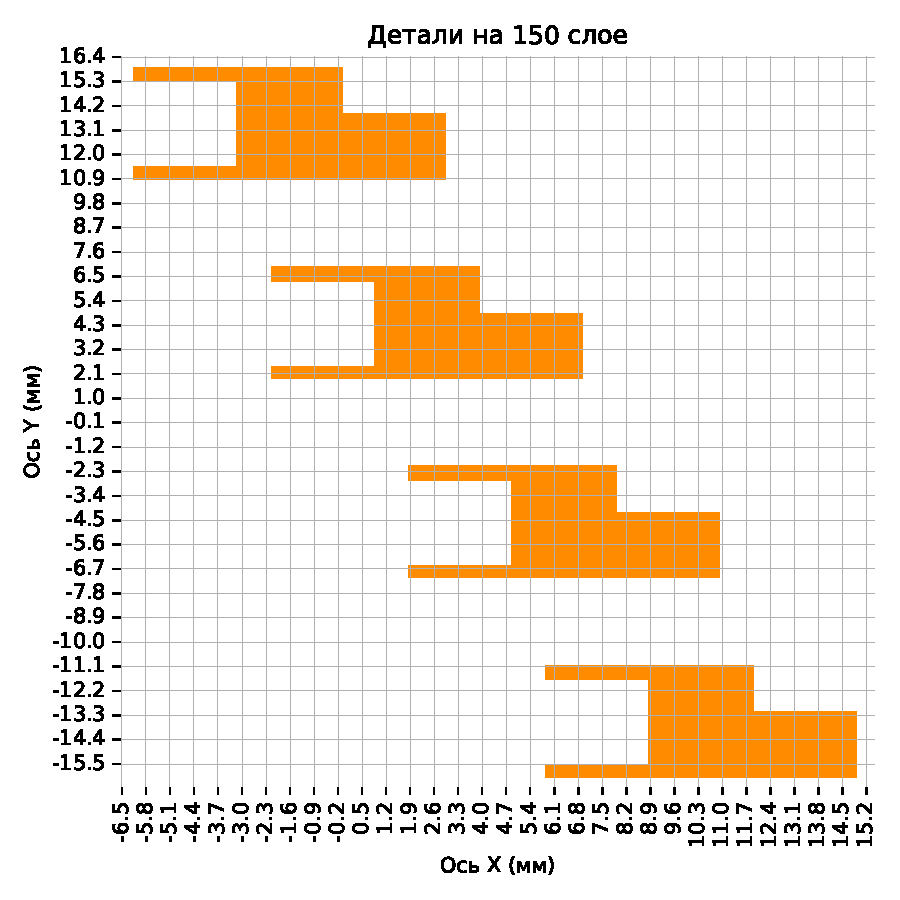
\includegraphics[scale=.4]{150_parts.pdf}
            \caption{Взаимное расположение деталей на слое №150.}
        \end{subfigure}
        \hfill
        \begin{subfigure}{.47\textwidth}
            \centering
            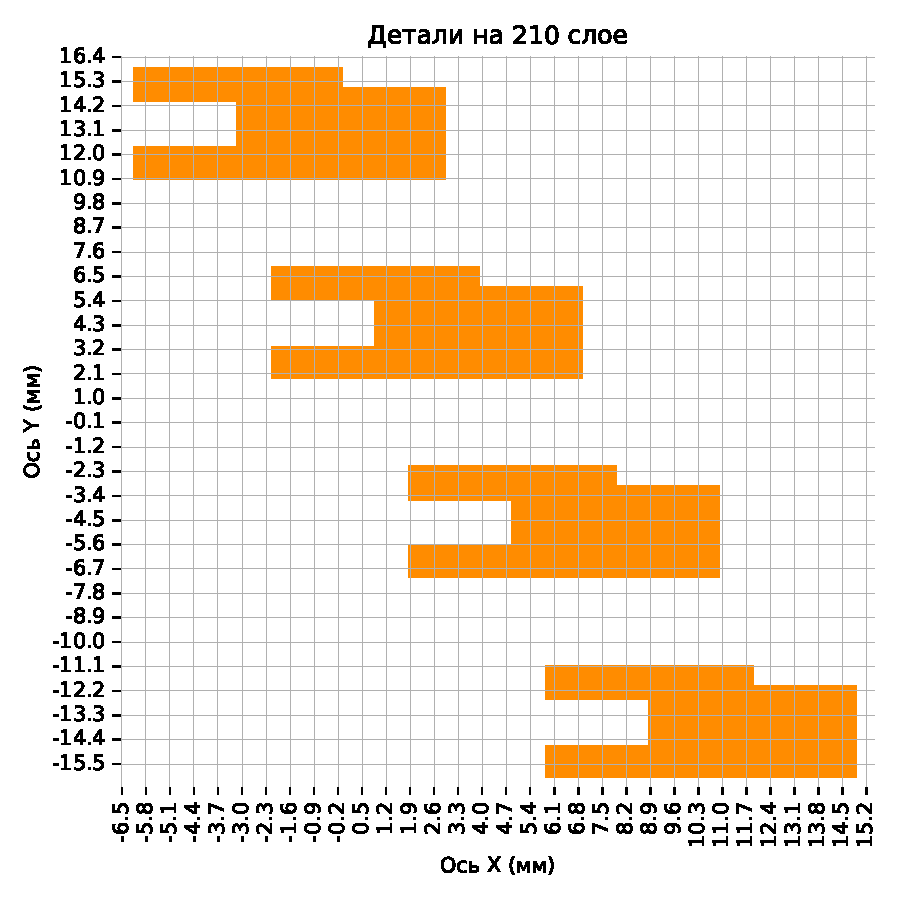
\includegraphics[scale=.4]{210_parts.pdf}
            \caption{Взаимное расположение деталей на слое №210.}
        \end{subfigure}
        \caption{Геометрия деталей на слоях №150 и №210.}\label{parts_geom}
    \end{figure}

    Изображения ванн расплава в наборе данных имеют размер $120 \times 120$ пикселей со значениями в диапазоне от 0 до 255. Каждый пиксель соответствует площади $8$~мкм~$\times$~$8$~мкм на лазерной установке. 

\subsection{Структуризация и предобработка данных}\label{struct}
    В связи с большим объёмом набора данных, было принято решение обучать модели на одном из 250 слоёв, и проводить валидацию на другом. Для обучения был выбран слой под номером 210, а для тестирования алгоритма -- слой №150, аналогично~\cite{convlstm_nist}. Первым шагом обработки выборки было полуавтоматическое определение некоторого количества аномальных изображений, согласно следующим правилам: \begin{itemize}
        \item Если на кадре присутствует несколько пятен соотносимого размера (это означает, что в данный момент произошёл всплеск, способный повлиять на качество детали)
        \item Если в последовательности подряд идущих кадров начинается резкое уменьшение/увеличение площади ванны расплава (это может означать, что произошла неполадка в работе установки или лазер начал двигаться по месту, где на детали остался дефект от одного из предыдущих проходов)
    \end{itemize} На Рис. \ref{anomaly_examples} и \ref{normal_examples} отображены соответственно аномальные и <<нормальные>> примеры ванн расплава, согласно описанному разделению.

    \begin{figure}[H]
        \centering
        \begin{subfigure}{.98\textwidth}
            \centering
            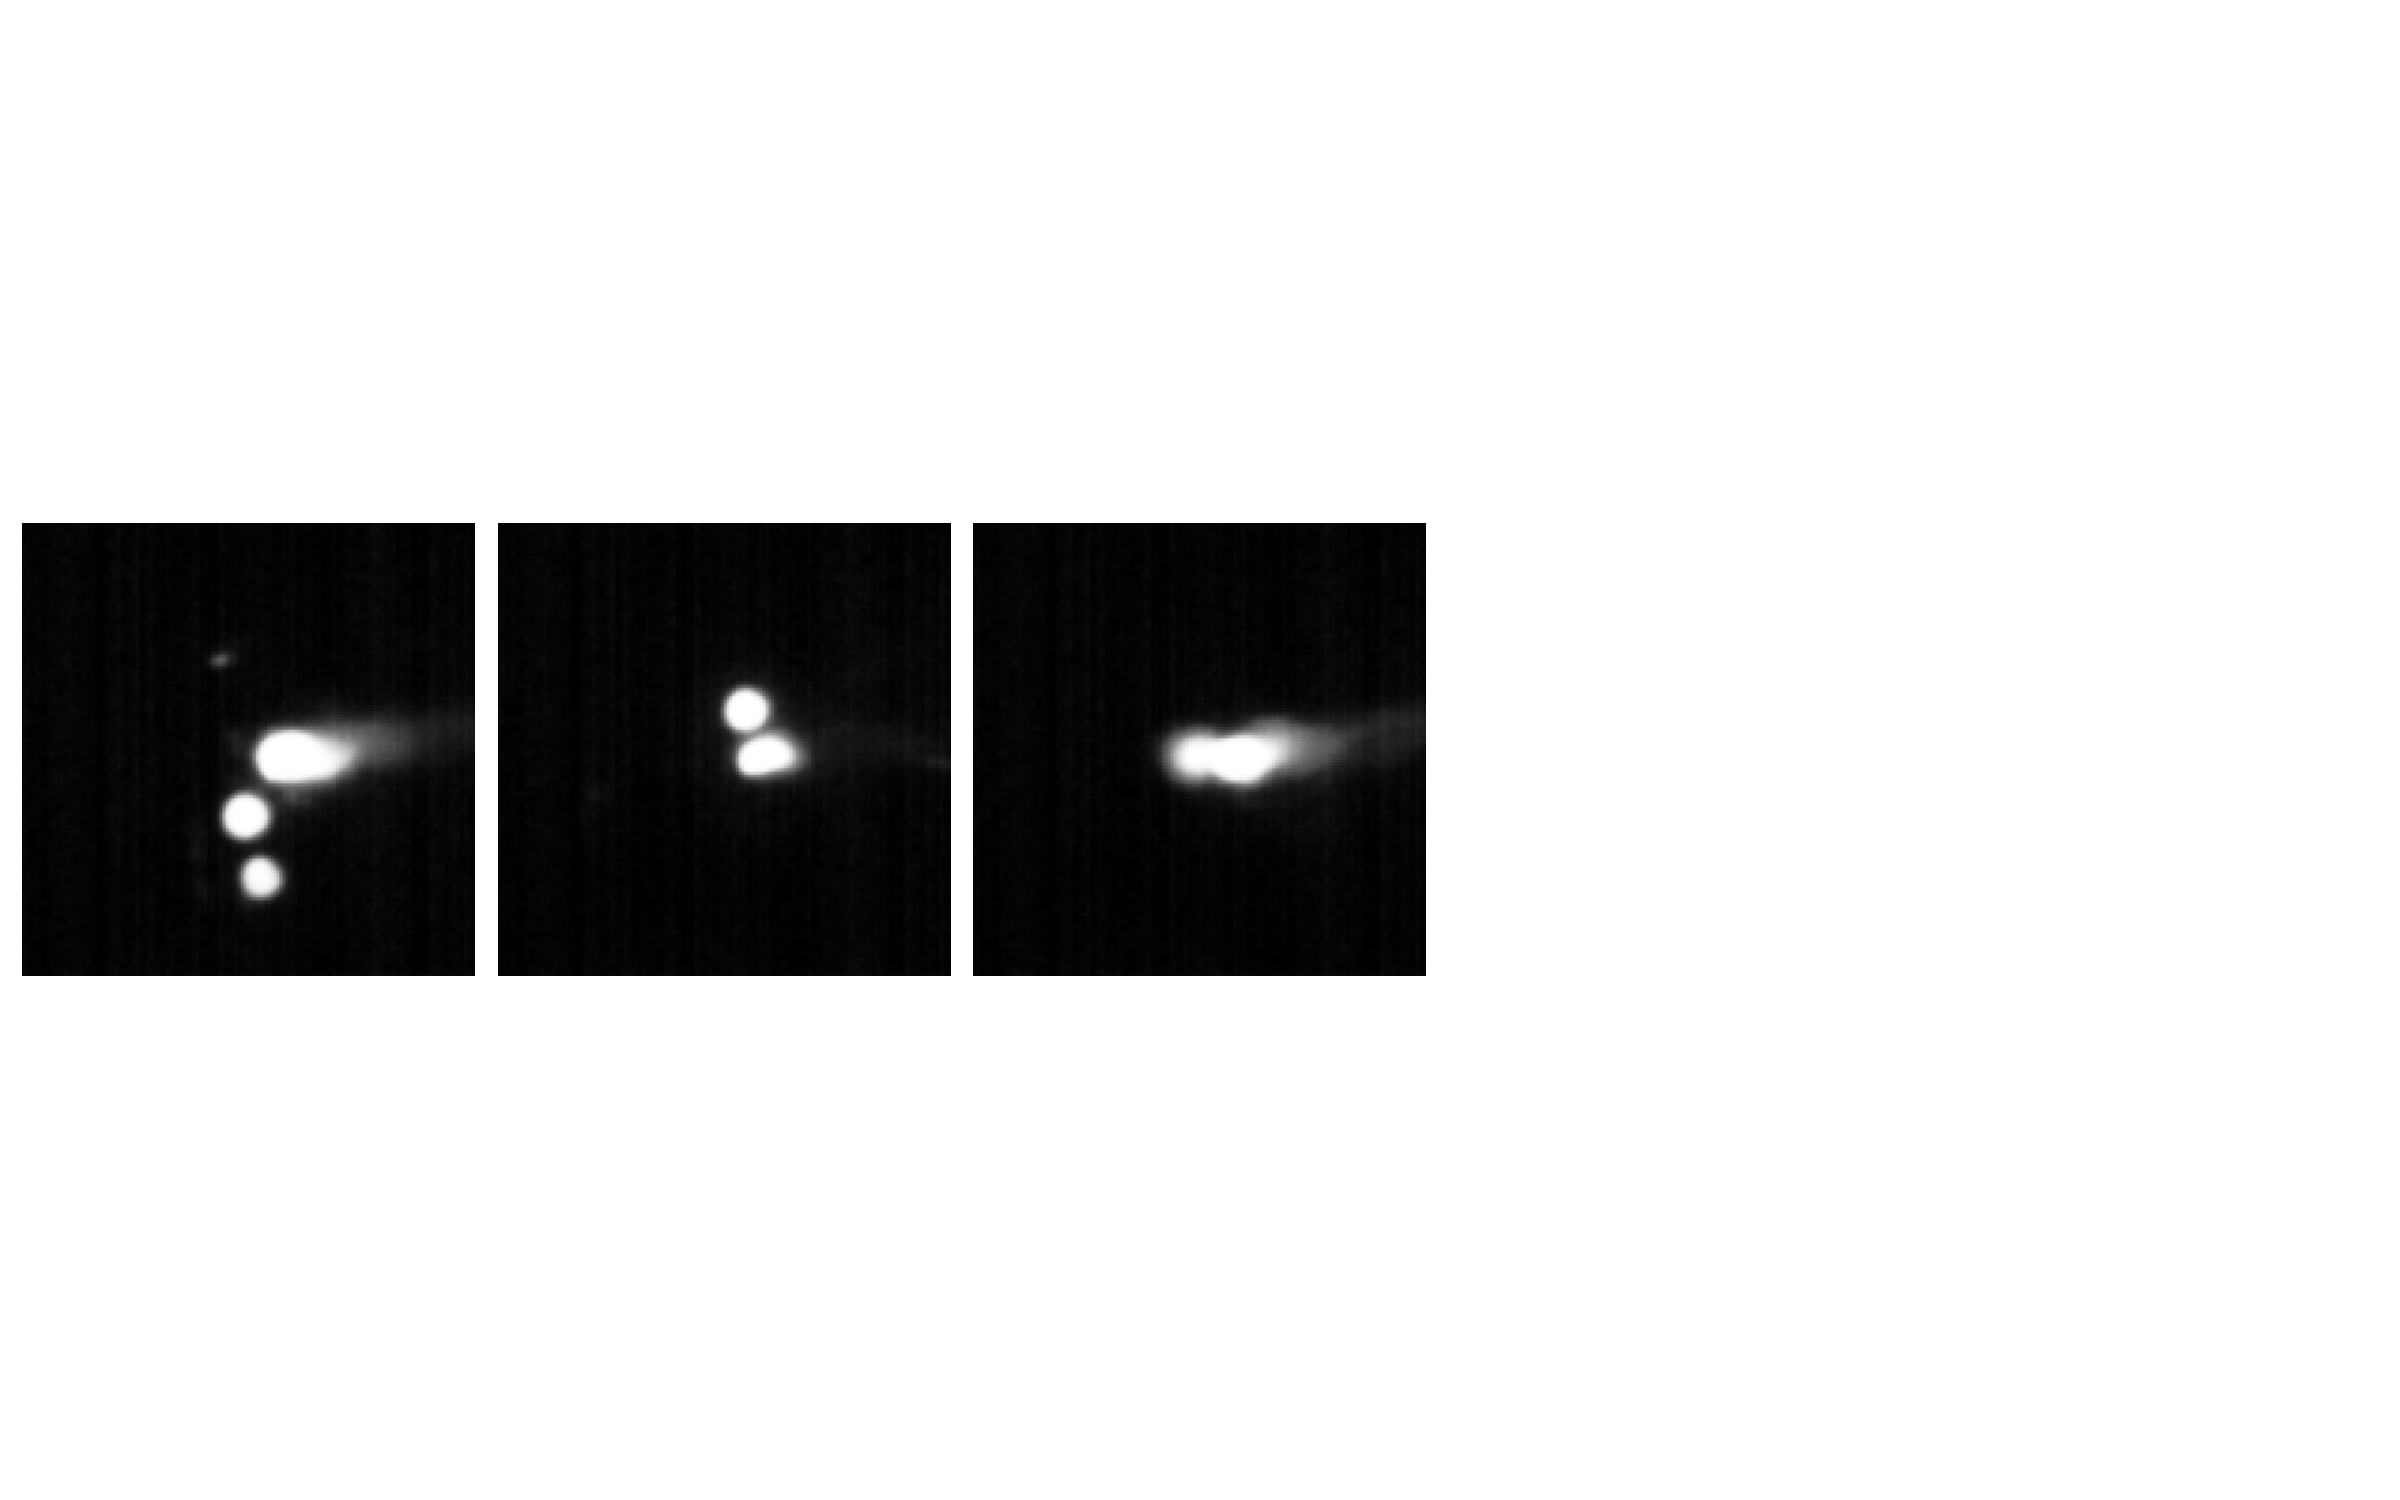
\includegraphics[scale=.5]{anomaly_examples.pdf}
            \caption{Примеры аномальных кадров.}\label{anomaly_examples}
        \end{subfigure}
        \\
        \centering
        \begin{subfigure}{.98\textwidth}
            \centering
            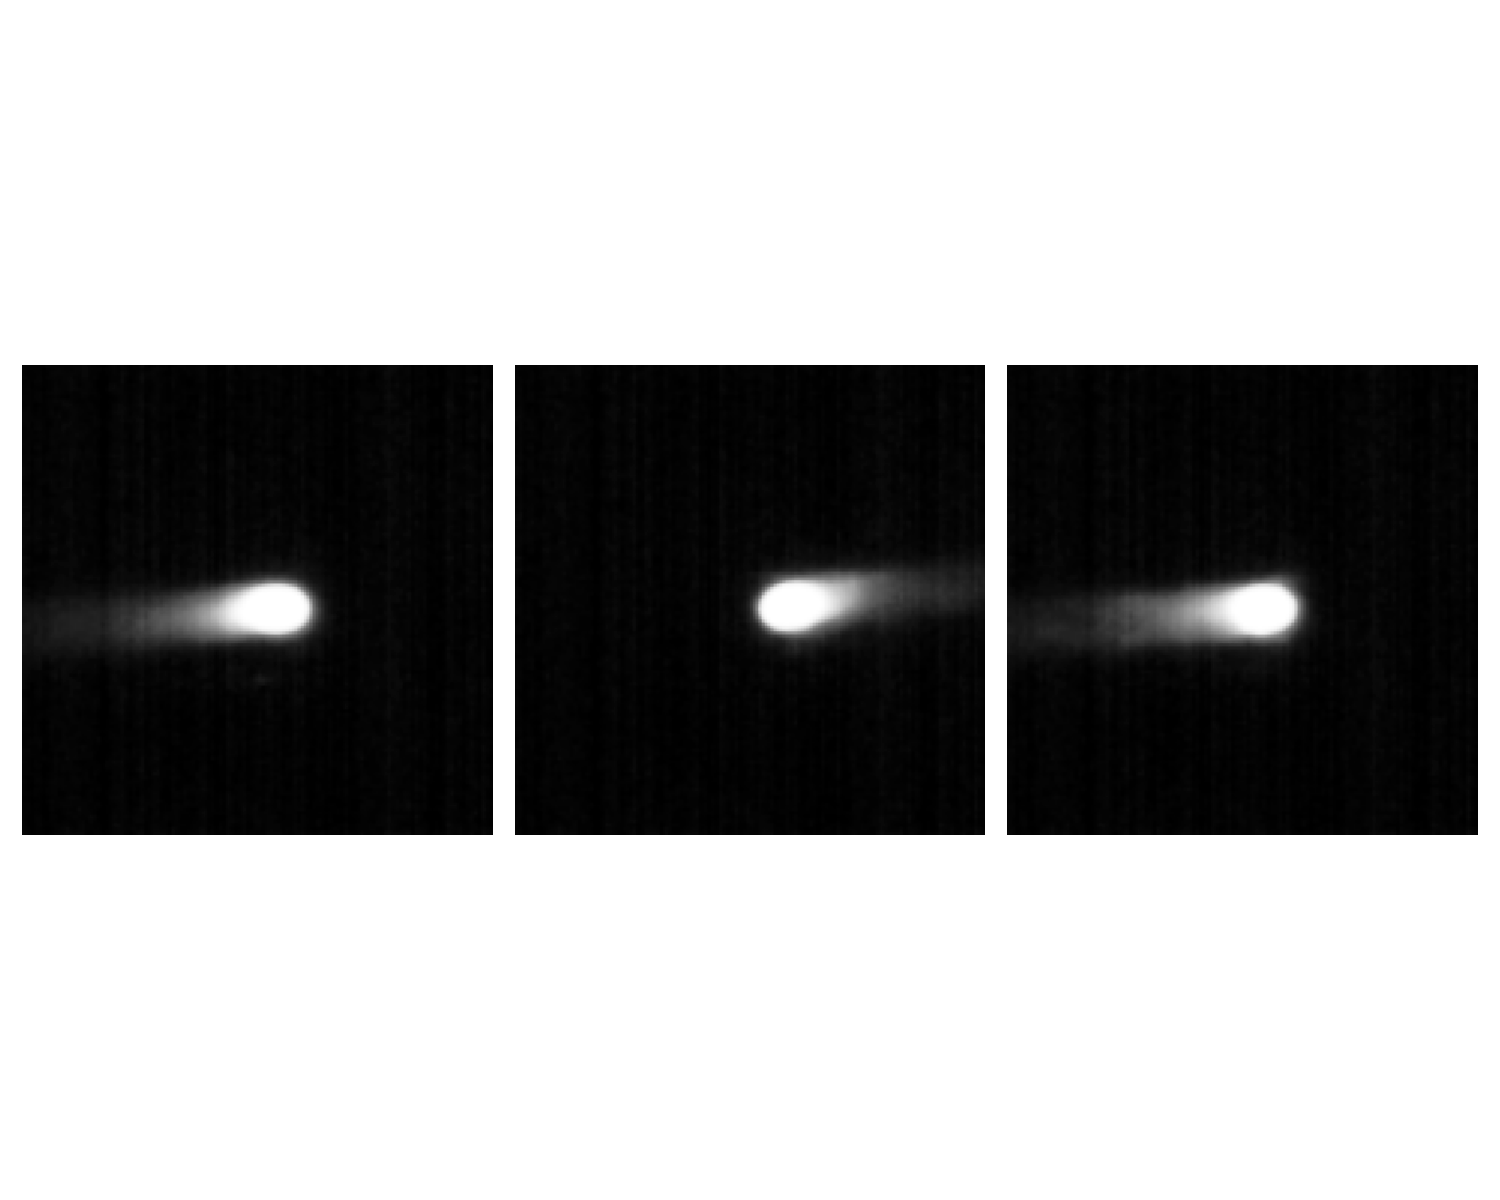
\includegraphics[scale=.48]{normal_examples.pdf}
            \caption{Примеры <<нормальных>> кадров.}\label{normal_examples}
        \end{subfigure}
        \caption{Примеры изображений ванн расплава.}\label{meltpool_examples}
    \end{figure}

    При подробном рассмотрении данных были обнаружены <<пустые>> кадры, на которых нет ванны расплава. Такие кадры встречаются на краях деталей (см. Рис. \ref{empties}), в связи с тем, что лазер заканчивает проход в одну сторону, и начинает в обратную. Подобные изображения тоже были отмечены как неподходящие для обучения.

    \begin{figure}[H]
        \center
        \begin{subfigure}{.47\textwidth}
            \centering
            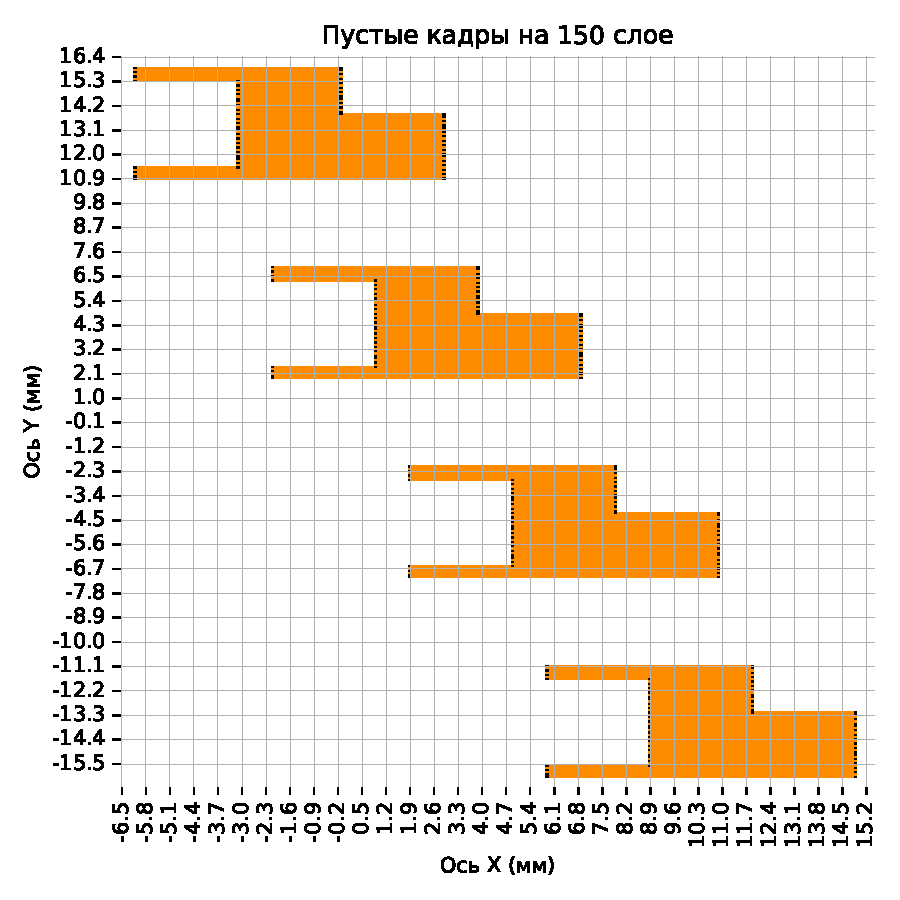
\includegraphics[scale=.55]{150_empties.pdf}
            \caption{<<Пустые>> кадры на слое №150.}
        \end{subfigure}
        \hfill
        \begin{subfigure}{.47\textwidth}
            \centering
            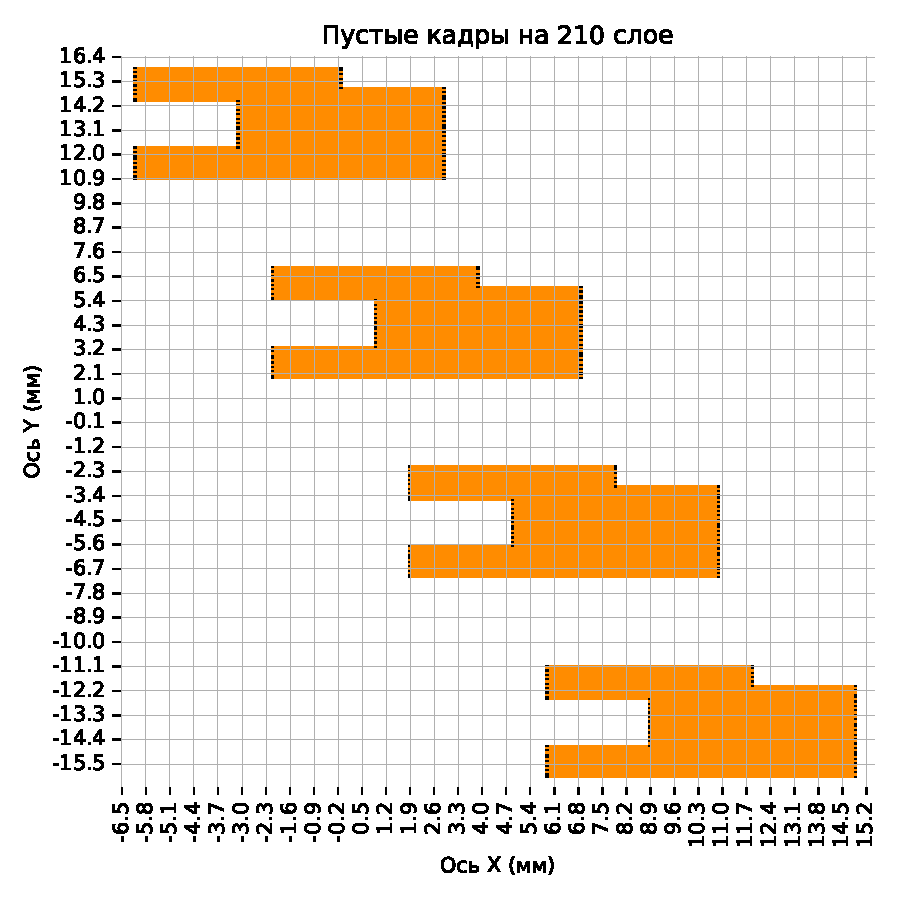
\includegraphics[scale=.55]{210_empties.pdf}
            \caption{<<Пустые>> кадры на слое №210.}
        \end{subfigure}
        \caption{Расположение <<пустых>> кадров на слоях №150 и №210, отмечены чёрным.}\label{empties}
    \end{figure}

    Все значения пикселей на изображениях были переведены в диапазон [$0.0$, $1.0$]. На вход моделям DL подавались последовательности из нескольких (фиксированное в пределах одной модели значение) подряд идущих во времени кадров, а в качестве прогноза ожидался кадр, следующий за входом. В связи с тем, что в обучающей выборке была помечена неподходящими для обучения часть изображений, вышеуказанные последовательности формировались следующим образом: если <<помеченный>> кадр попадал в последовательность или следовал сразу за ней, то такая последовательность исключалась из тренировочного набора данных. Полученные таким образом выборки будем называть далее по номеру соответствующего слоя с приписанной буквой \textbf{A} (\textit{Пример:} набор данных \textbf{150A}).

    В качестве аугментаций, для повышения обобщающей способности моделей, были использованы следующие приёмы: поворот всей последовательности кадров (включая следующий за ней предсказываемый кадр) на угол из диапазона [$-2\pi$, $2\pi$], и изменение масштаба в диапазоне [$70\%$, $130\%$].

    В дальнейшем для получения лучшей модели был использован следующий подход: производилось обучение алгоритма на полученных в результате применения вышеописанных шагов данных, а потом по порогу на функционал ошибки восстановления \eqref{mse} из обучающей выборки аналогичным образом удалялись последовательности, определённые полученной моделью как аномальные. Полученные в результате этих действий данные будем обозначать по номеру слоя с приписанной буквой \textbf{B} (\textit{Пример:} набор данных \textbf{210B}). Затем новая модель обучалась на вновь очищенном от аномалий наборе данных.
    

\section{Существующий подход}
    В качестве первого метода была рассмотрена модель ConvLSTMAE~\cite{convlstm_nist} -- автокодировщика, основанного на архитектуре свёрточной LSTM~\cite{convlstm_arch}. Такая архитектура позволяет успешно использовать последовательную структуру данных, являющихся при этом двумерными сигналами. Подробное описание архитектуры использовавшейся нейронной сети можно наблюдать в Приложении \ref{app:archs}. Обучение производилось с помощью оптимизатора AdamW~\cite{adamw} с темпом обучения равным $10^{-3}$ и с использованием функции потерь бинарной кросс-энтропии: \begin{equation}\label{BCE}
        BCELoss(X, \hat{X}) := -\sum\limits_{i, j}\left(X_{ij}\log{\hat{X}_{ij}} + (1 - X_{ij})\log{(1 - \hat{X}_{ij})}\right),
    \end{equation}где $X$ -- матрица целевого кадра, а $\hat{X}$ --предсказанного. Размер мини-батча был выбран равным 16, обучение проводилось на протяжении 20 эпох. Данные гиперпараметры обучения моделей были зафиксированы для всех алгоритмов на протяжении всего исследования.
\subsection{Эксперименты}
    Согласно описанному выше подходу, сначала производилось обучение на выборке \textbf{210A} с проведением валидации на наборе данных \textbf{150A}. Для первой модели было зафиксировано значение числа кадров в последовательности равное 4. На Рис. \ref{model_4_train_worst} и \ref{model_4_test_worst} изображены примеры из соответственно тренировочного и валидационного наборов худших по значению функционала ошибки восстановления кадров.

    \begin{figure}[H]
        \centering
        \begin{subfigure}{.47\textwidth}
            \centering
            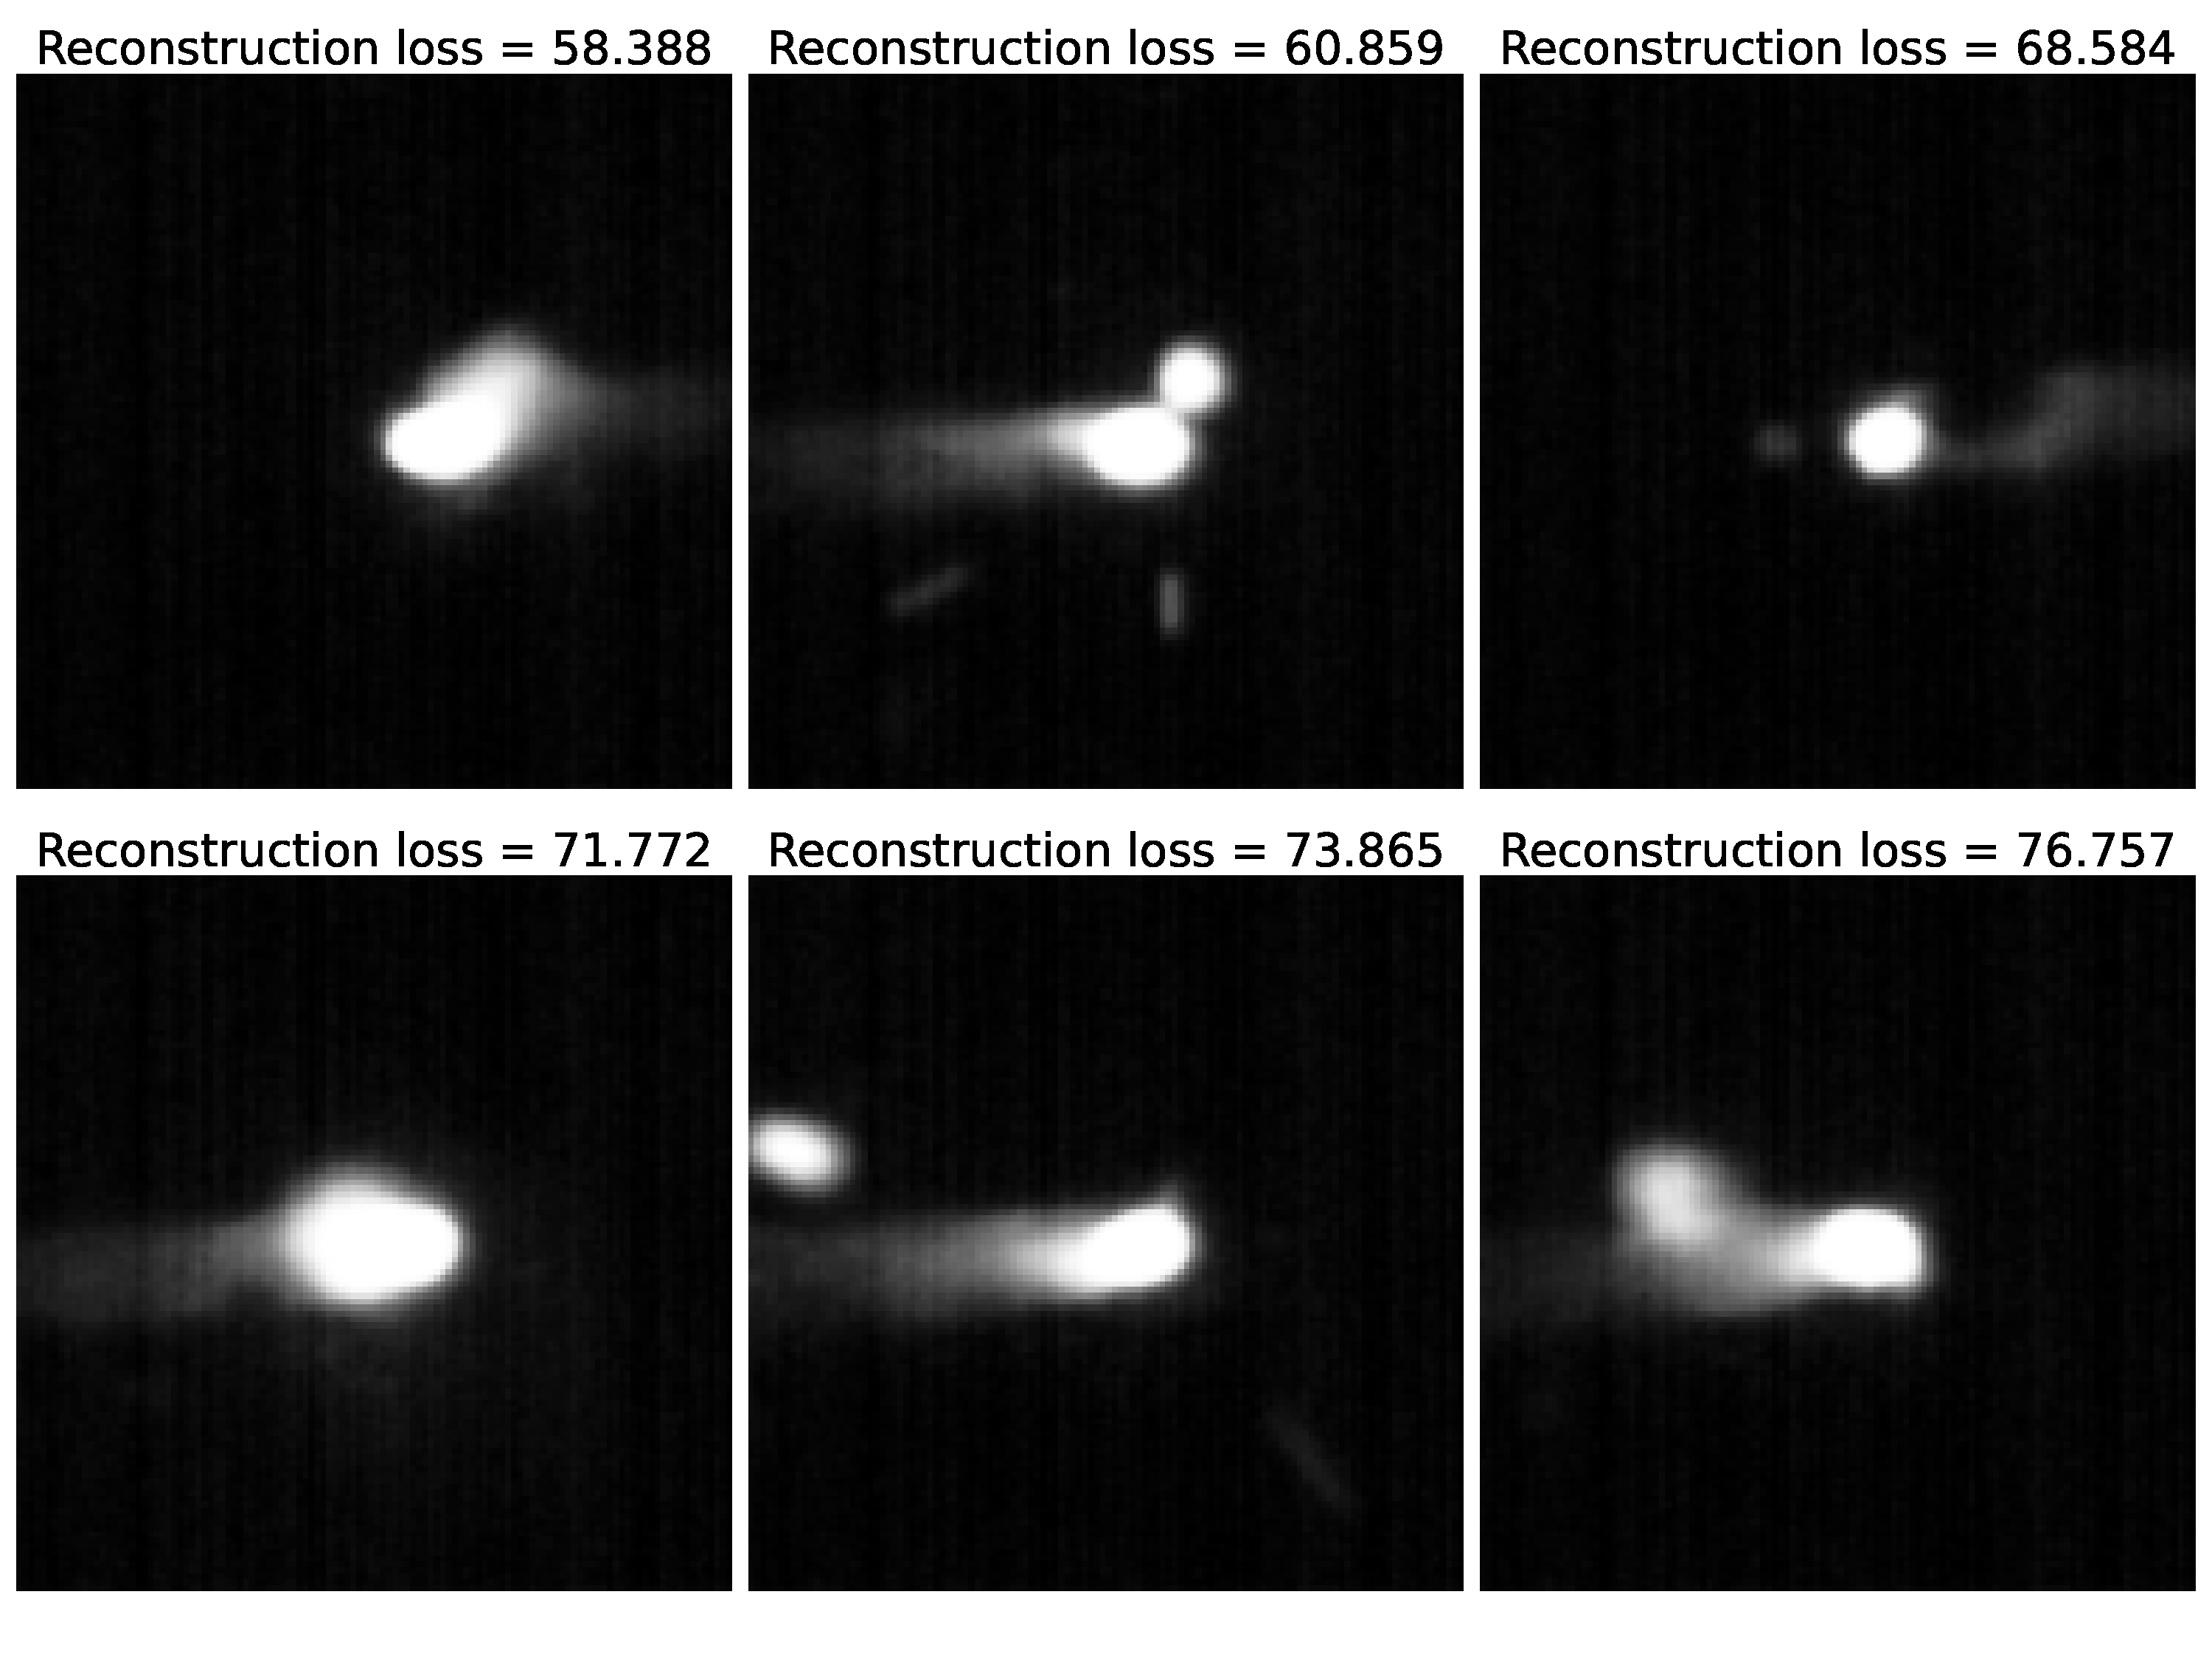
\includegraphics[scale=.15]{model_4_train_worst.pdf}
            \caption{Примеры худших по значению функционала ошибки восстановления кадров из тренировочного набора \textbf{210A}.}\label{model_4_train_worst}
        \end{subfigure}
        \hfill
        \begin{subfigure}{.47\textwidth}
            \centering
            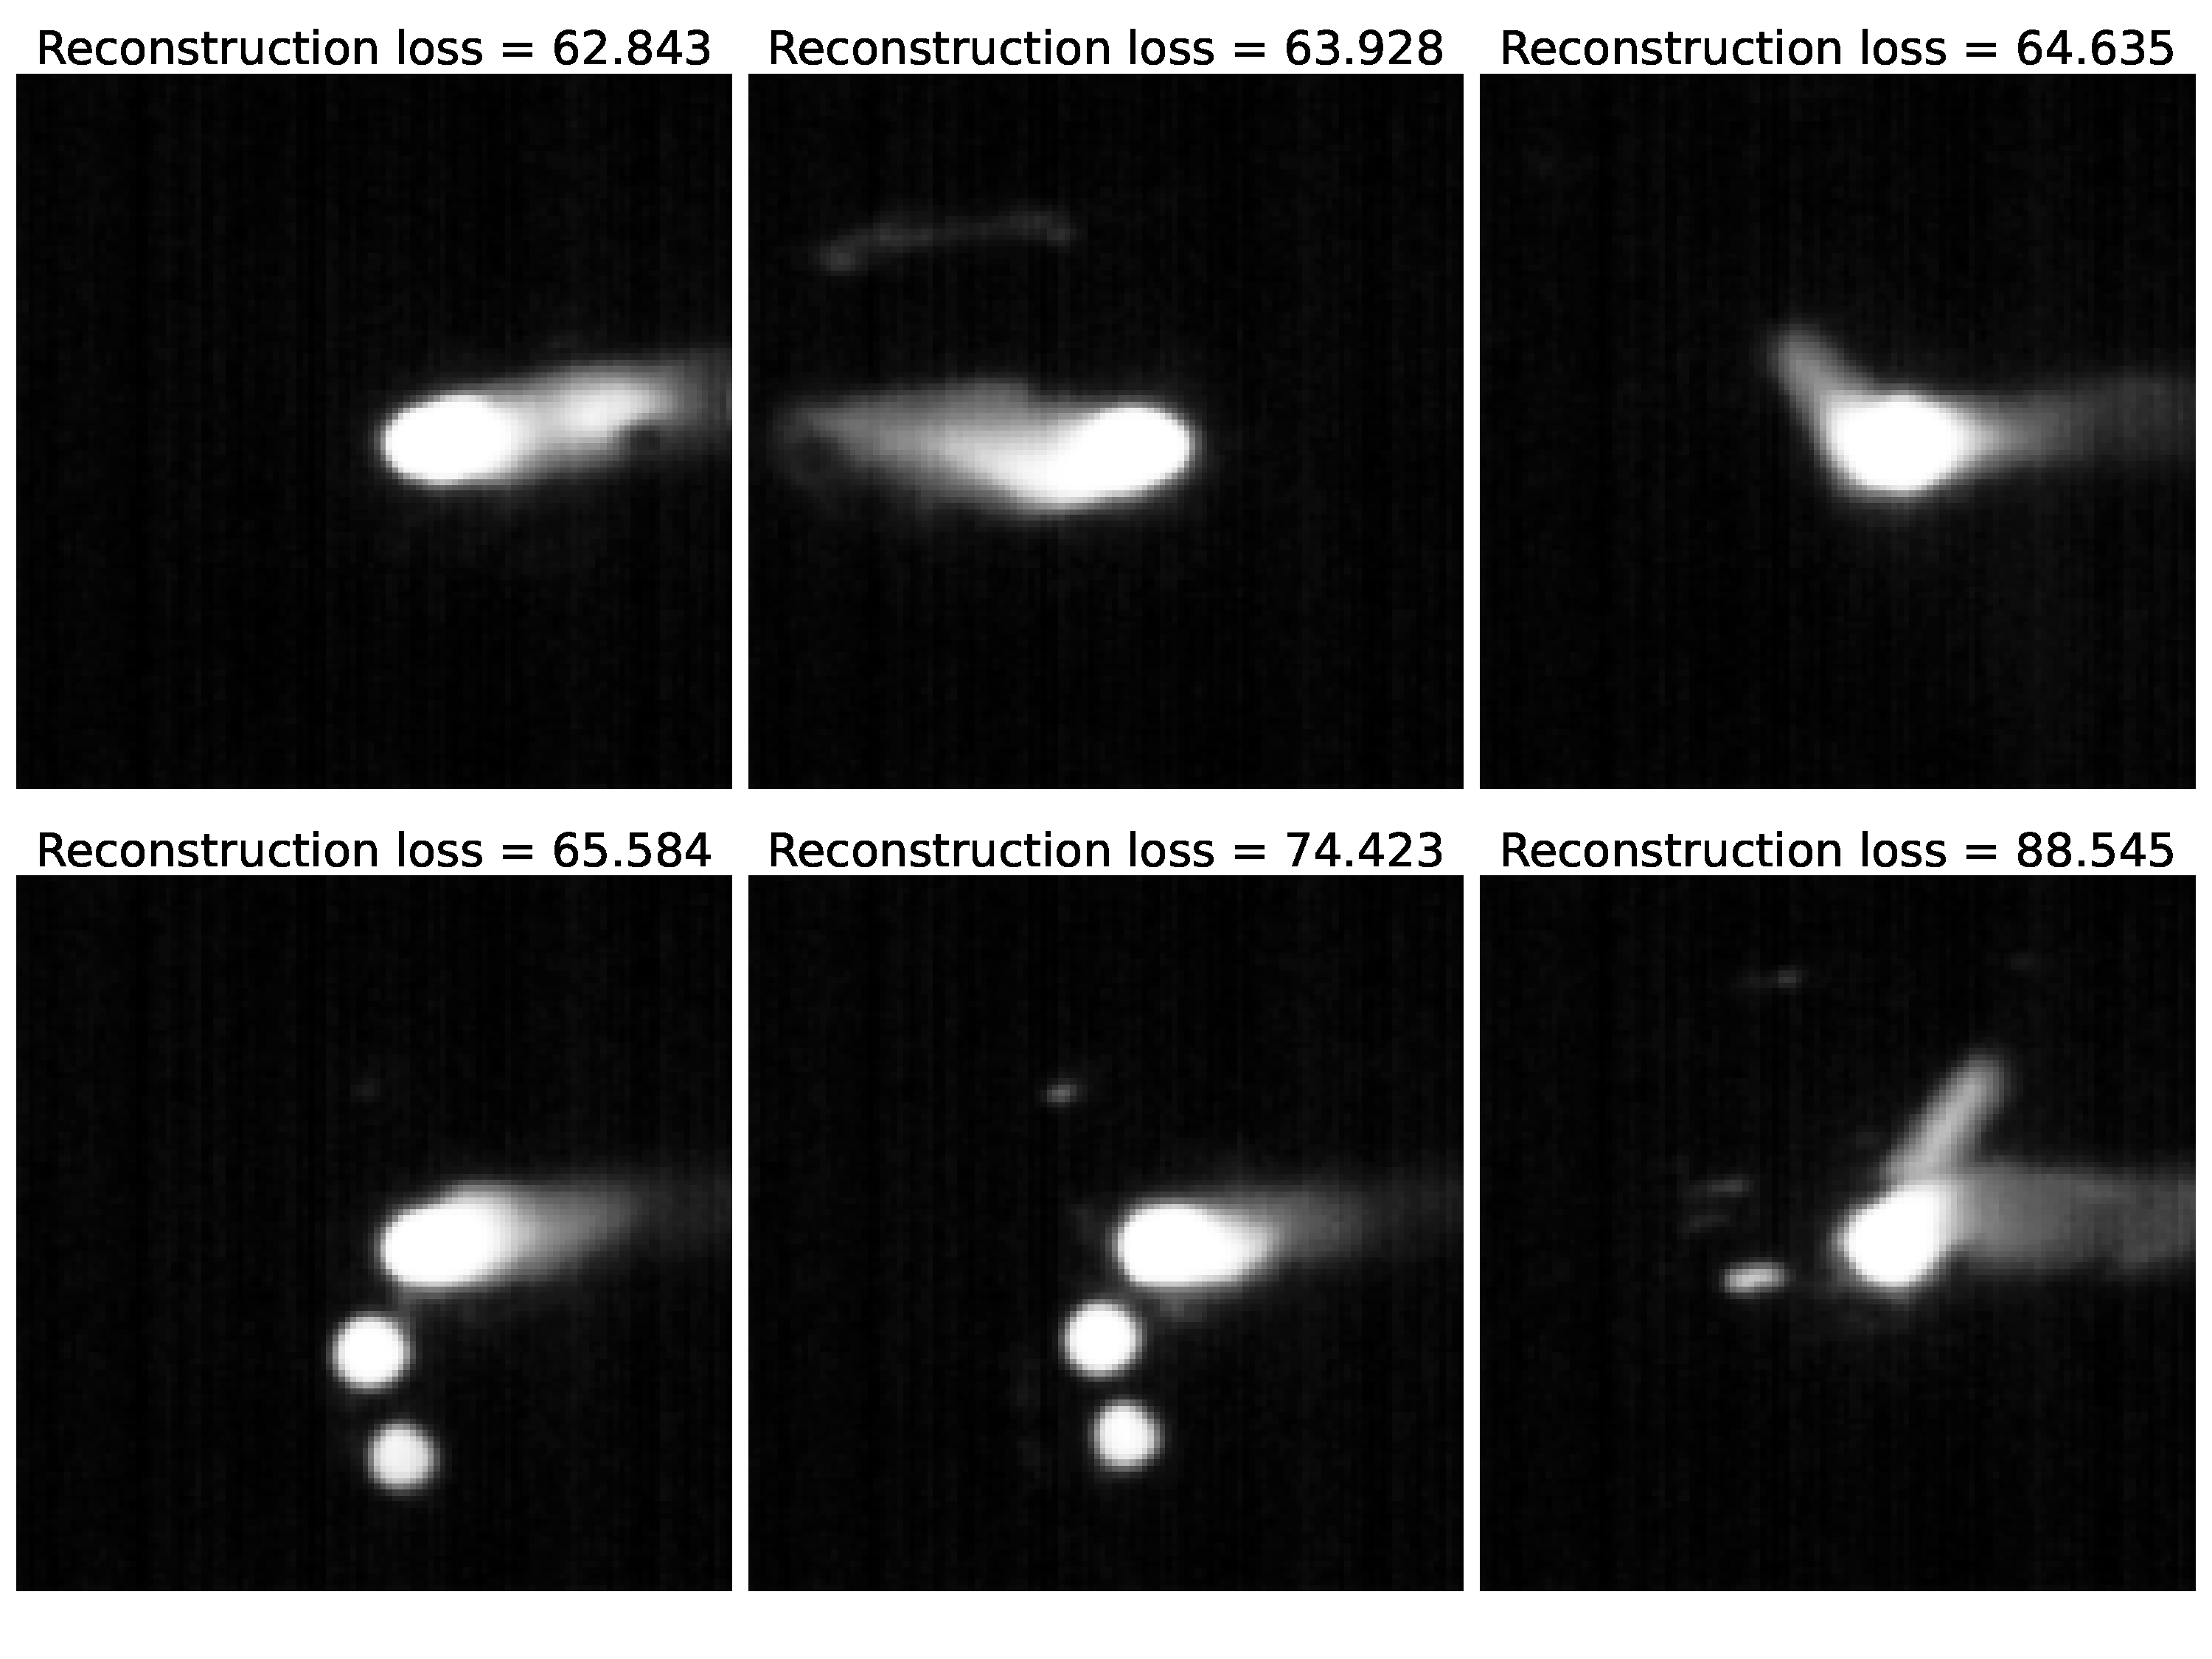
\includegraphics[scale=.15]{model_4_test_worst.pdf}
            \caption{Примеры худших по значению функционала ошибки восстановления кадров из валидационного набора \textbf{150A}.}\label{model_4_test_worst}
        \end{subfigure}
        \caption{Примеры найденных ConvLSTMAE, обученной на \textbf{210A} с размером окна 4, аномальных кадров. Над изображениями подписано значение функционала ошибки восстановления \eqref{mse}.}\label{lstm_worst_before}
    \end{figure}

    На Рис. \ref{model_4_loss_distr} изображена плотность распределения значения функционала ошибки восстановления полученной модели на обучающей и на тестовой выборках, и отмечено значение 99-го перцентиля значения SE \eqref{mse} на тренировочном наборе данных.

    \begin{figure}[]
        \centering
        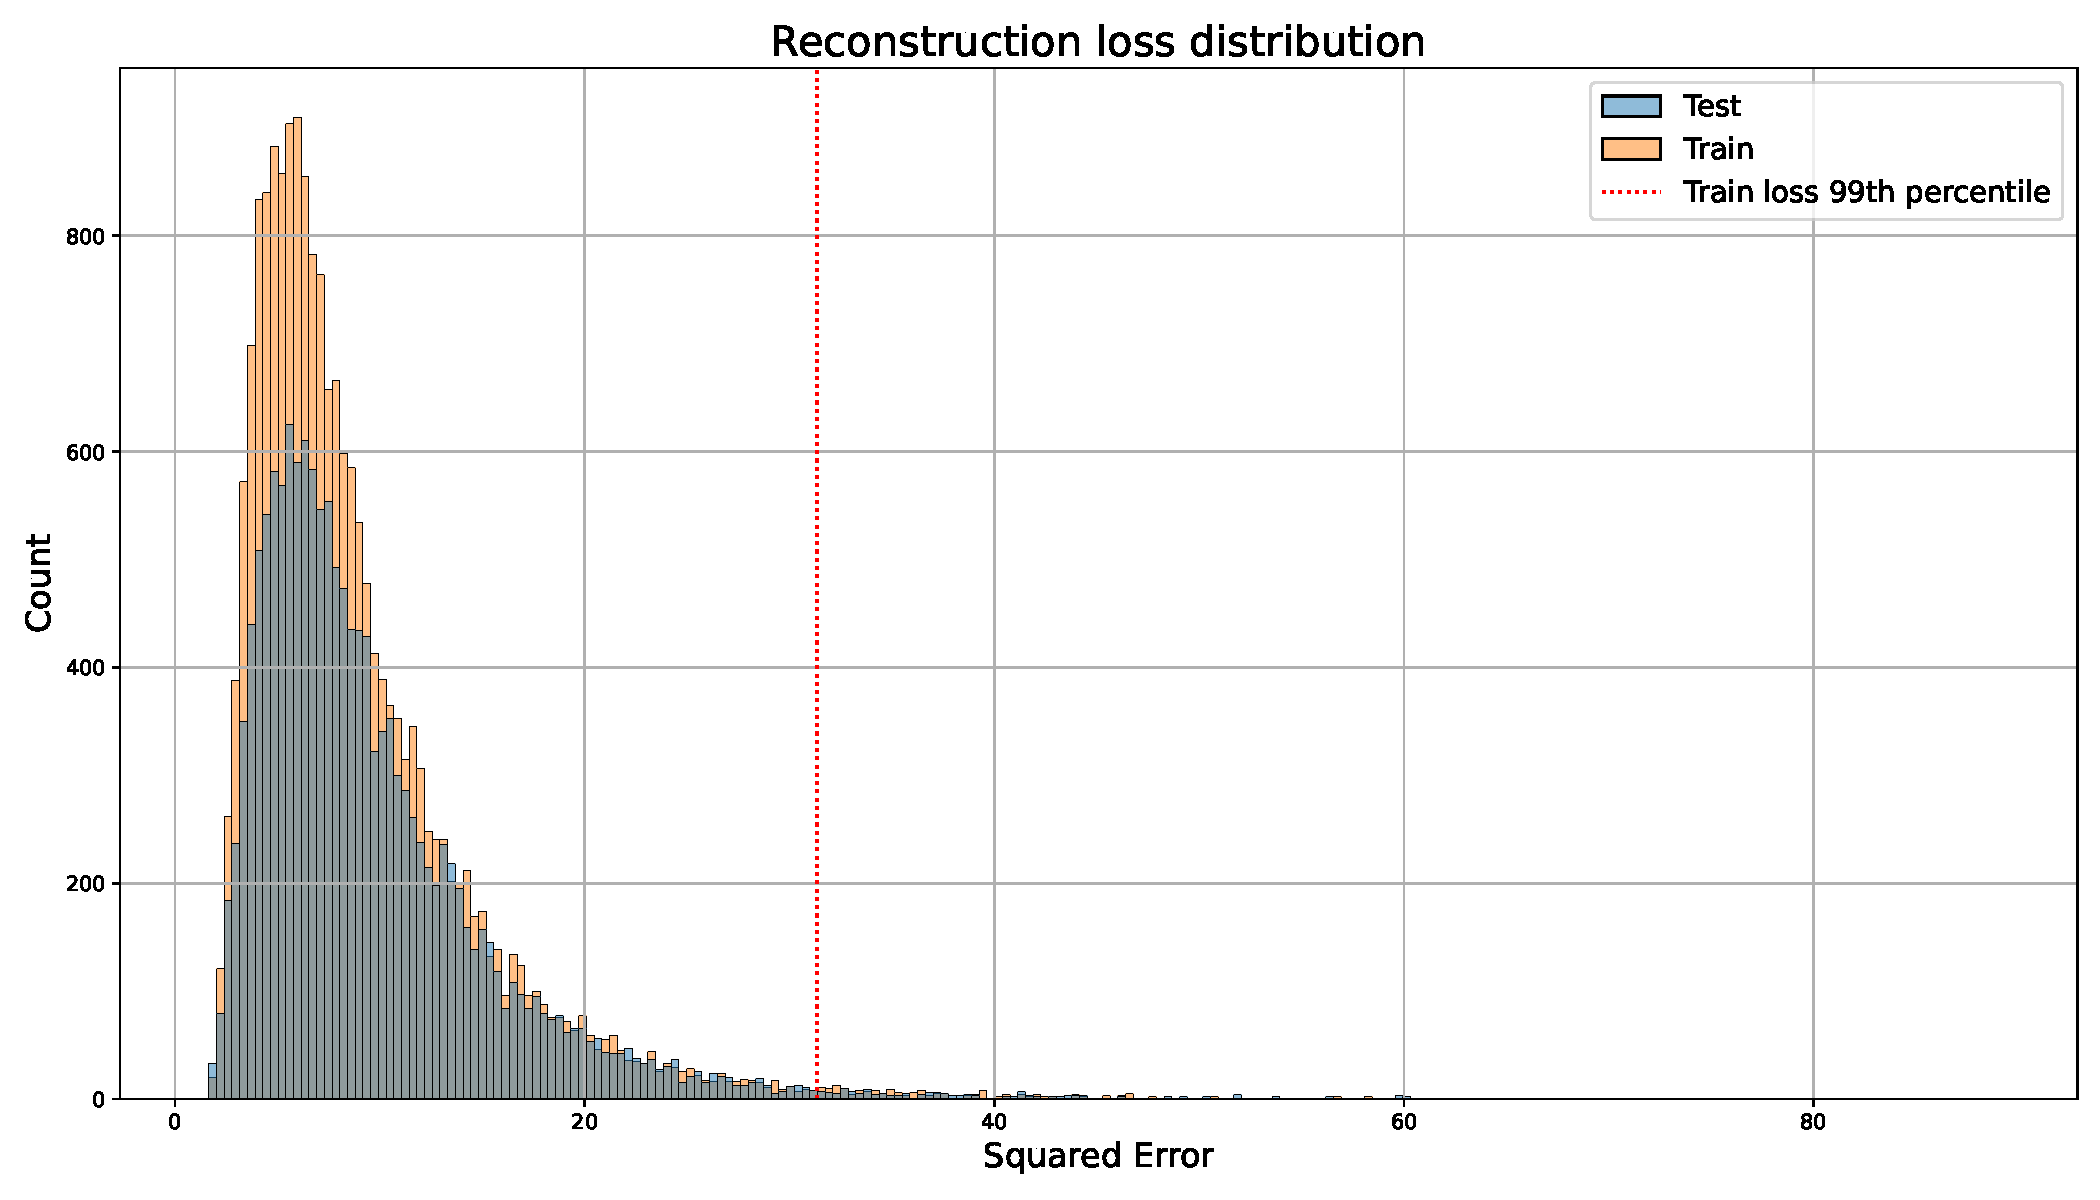
\includegraphics[scale=0.3]{model_4_loss_distr.pdf}
        \caption{Распределение значений функционала \eqref{mse} на обучающей и валидационной выборке для модели ConvLSTMAE, обученной на \textbf{210A} при значении размера окна равном 4.}
        \label{model_4_loss_distr}
    \end{figure}

    Видно, что плотности на обучающей и валидационной выборках мало отличаются по <<форме>>, что говорит о присутствии генерализации модели и оправданности её применения для мониторинга в течение всего процесса плавления. При этом заметно, что распределение имеет <<тяжёлый хвост>>, что может говорить о том, что модель имеет сравнительно высокую ошибку на объектах, не являющихся аномальными.

    На Рис. \ref{lstm_xy_before} отображены значения функционала ошибки восстановления для различных координат положения лазера в момент запечатления ванны расплава. В связи с пустыми кадрами, появляющимися при изменении направления движения лазера на $180\degree$, для таких последовательностей предсказания не были учтены во избежание смещения фокуса рассмотрения на места с заведомо большим значением ошибки. Координаты ванн расплава взяты с округлением в $0.1$ мм, проведено усреднение значений функционала ошибки по координате. В связи со спецификой выбранного валидационного набора данных, на Рис. \ref{lstm_4_window_xy_test_before} можно заметить больше аномальных значений функционала ошибки, чем на Рис. \ref{lstm_4_window_xy_train_before}. 

    \begin{figure}[H]
        \centering
        \begin{subfigure}{.47\textwidth}
            \centering
            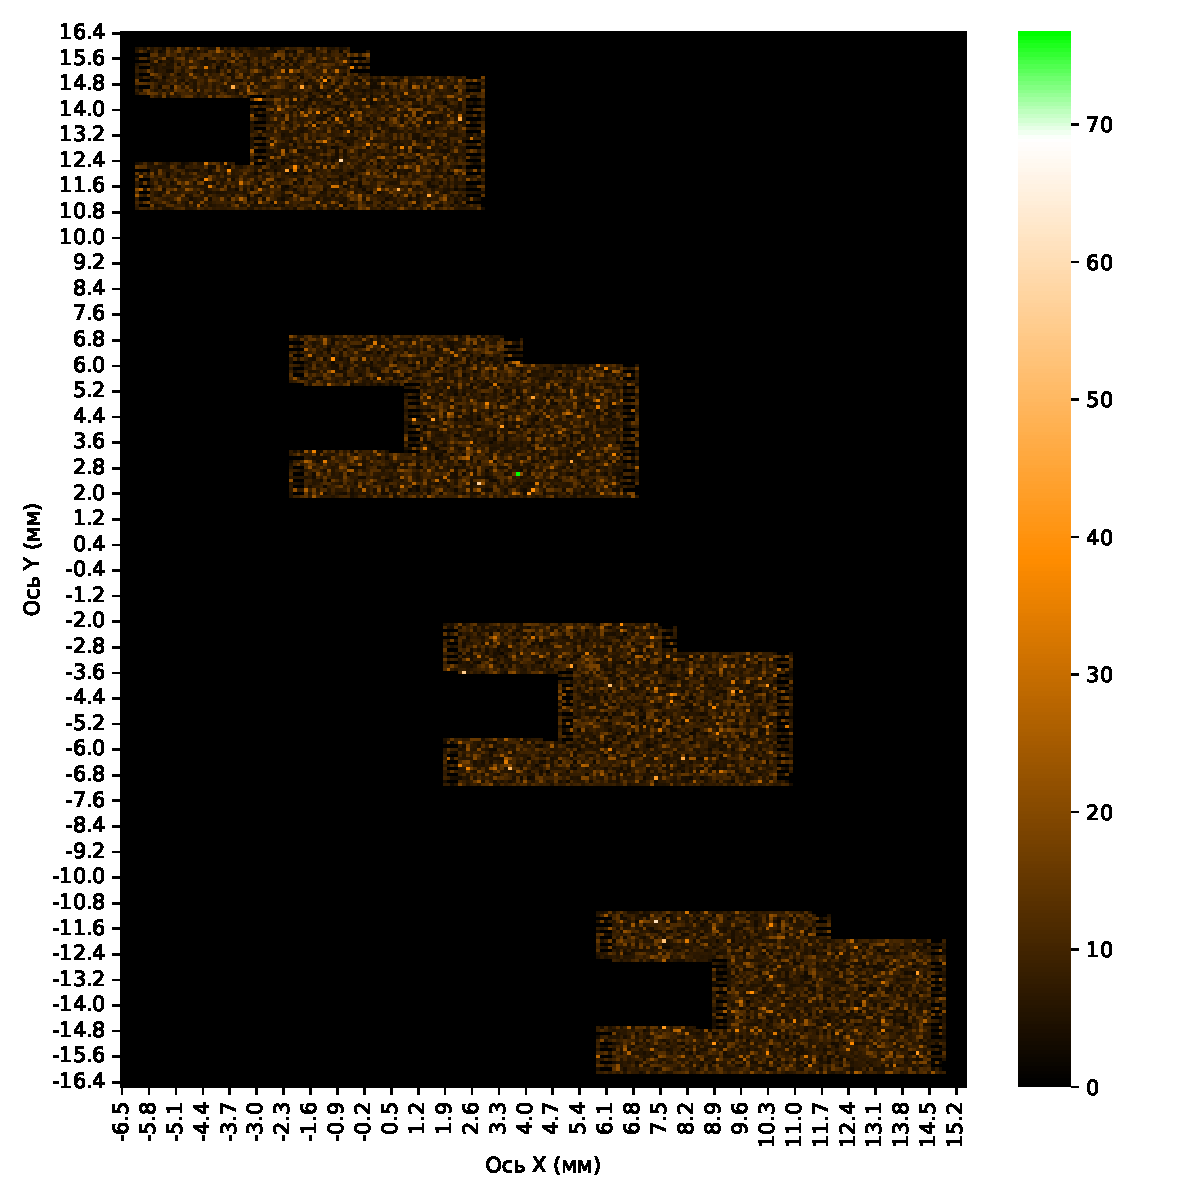
\includegraphics[scale=.35]{lstm_4_window_xy_train_before.pdf}
            \caption{Среднее по координате значение функционала ошибки восстановления для тренировочного набора \textbf{210A}.}\label{lstm_4_window_xy_train_before}
        \end{subfigure}
        \hfill
        \begin{subfigure}{.47\textwidth}
            \centering
            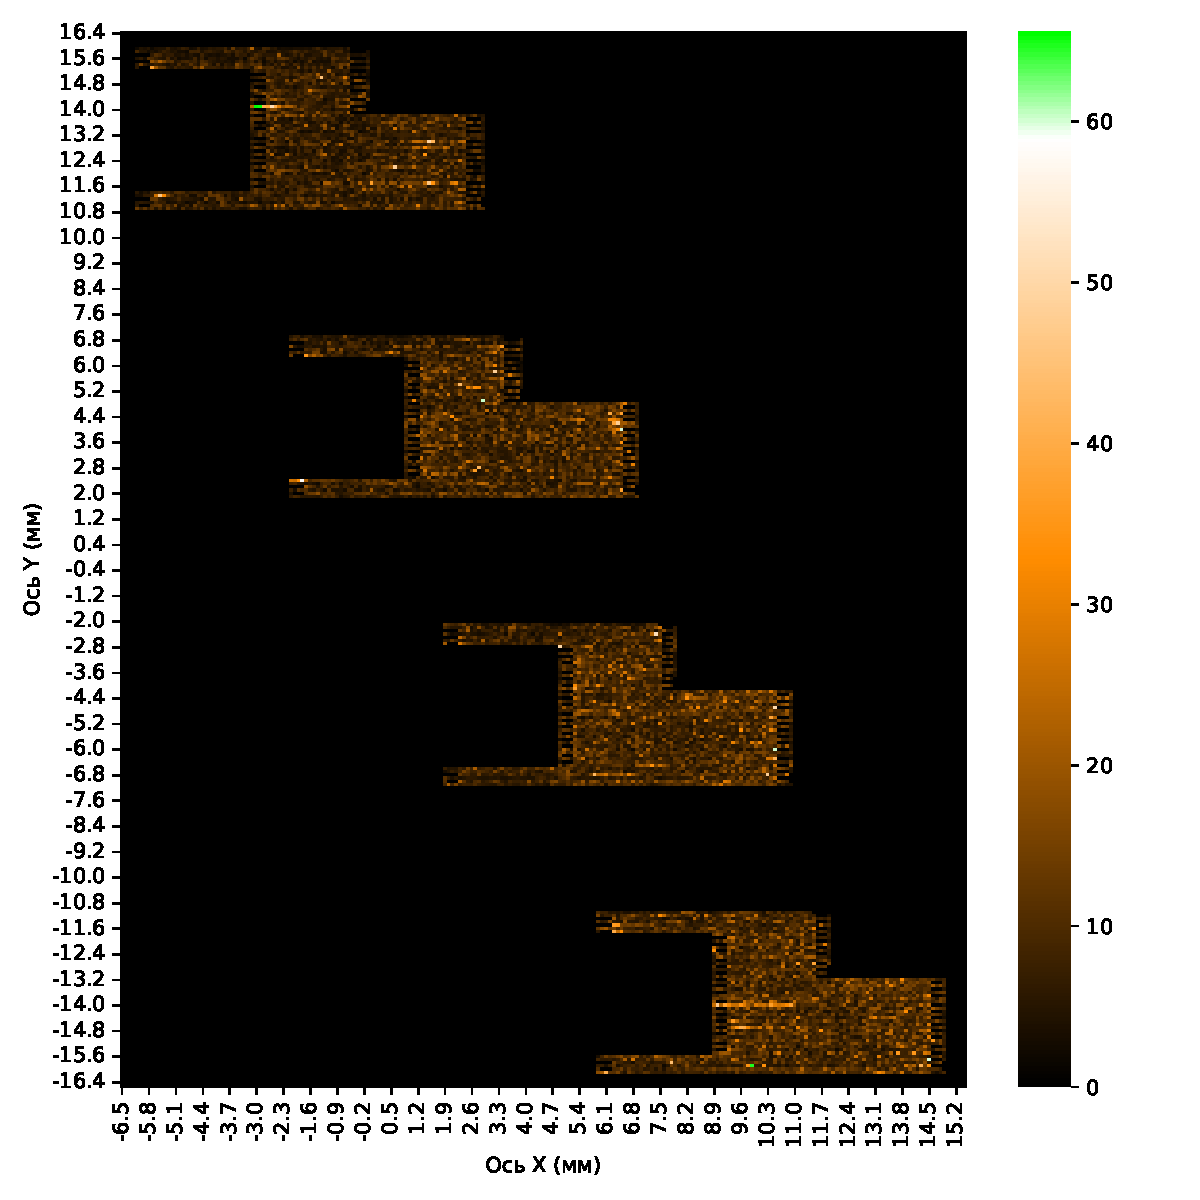
\includegraphics[scale=.35]{lstm_4_window_xy_test_before.pdf}
            \caption{Среднее по координате значение функционала ошибки восстановления для валидационного набора \textbf{150A}.}\label{lstm_4_window_xy_test_before}
        \end{subfigure}
        \caption{Распределение функционала \eqref{mse} по координате для модели ConvLSTMAE, обученной на \textbf{210A} с размером окна 4.}\label{lstm_xy_before}
    \end{figure}

    Такое представление позволяет сказать больше о возможных нарушениях производимого процесса печати. Например, на области, в которой в среднем происходит много аномалий, может оказаться дефективное наплавление, которое будет оказывать влияние на технологический процесс на протяжении нескольких последующих слоёв. В таком случае необходимо останавливать процесс печати для исправления ситуации или прекращения работы в случае неисправимой ошибки во избежание потерь времени и материалов на производство заведомо бракованной детали.

    Для проведения второй части описанного метода обучения модели, по алгоритму из подраздела \ref{struct} из набора данных \textbf{210A} были удалены 1000 объектов, являющихся худшими по значению функционала ошибки восстановления для модели ConvLSTMAE с размером окна 4. 

    \begin{figure}[]
        \centering
        \begin{subfigure}{.47\textwidth}
            \centering
            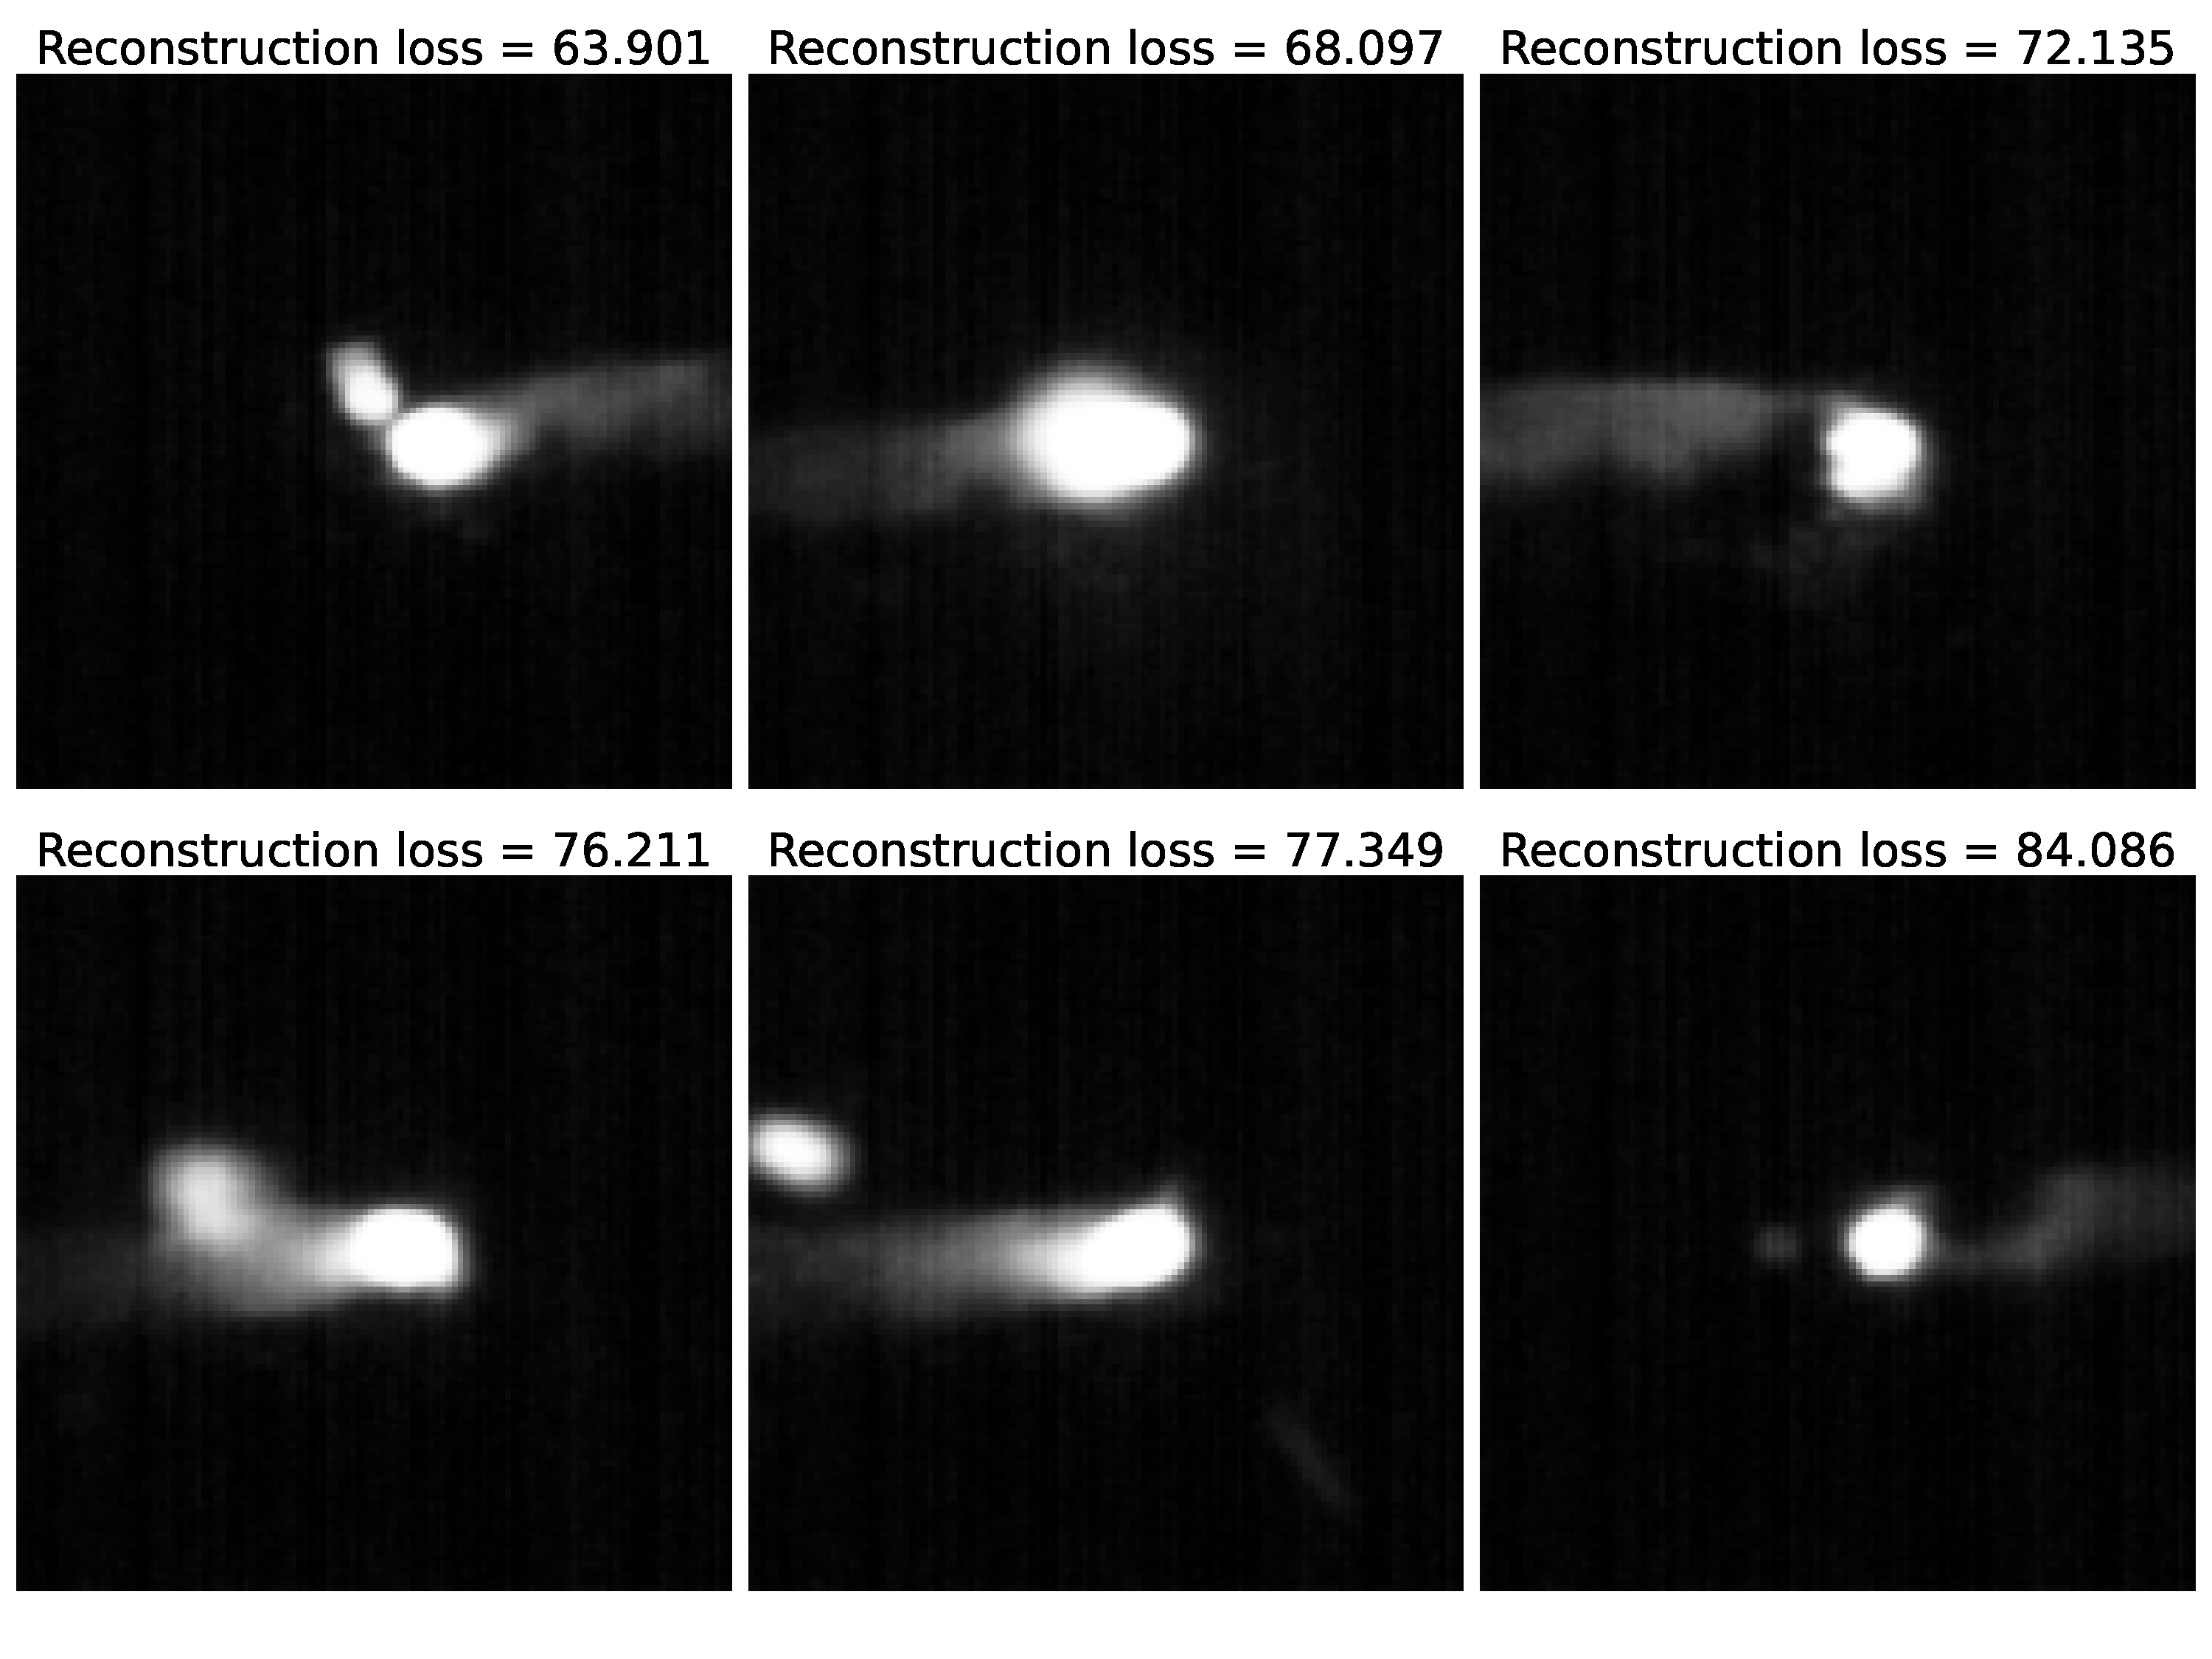
\includegraphics[scale=.15]{model_4_after_train_worst.pdf}
            \caption{Примеры худших по значению функционала ошибки восстановления кадров из тренировочного набора \textbf{210B}.}\label{model_4_after_train_worst}
        \end{subfigure}
        \hfill
        \begin{subfigure}{.47\textwidth}
            \centering
            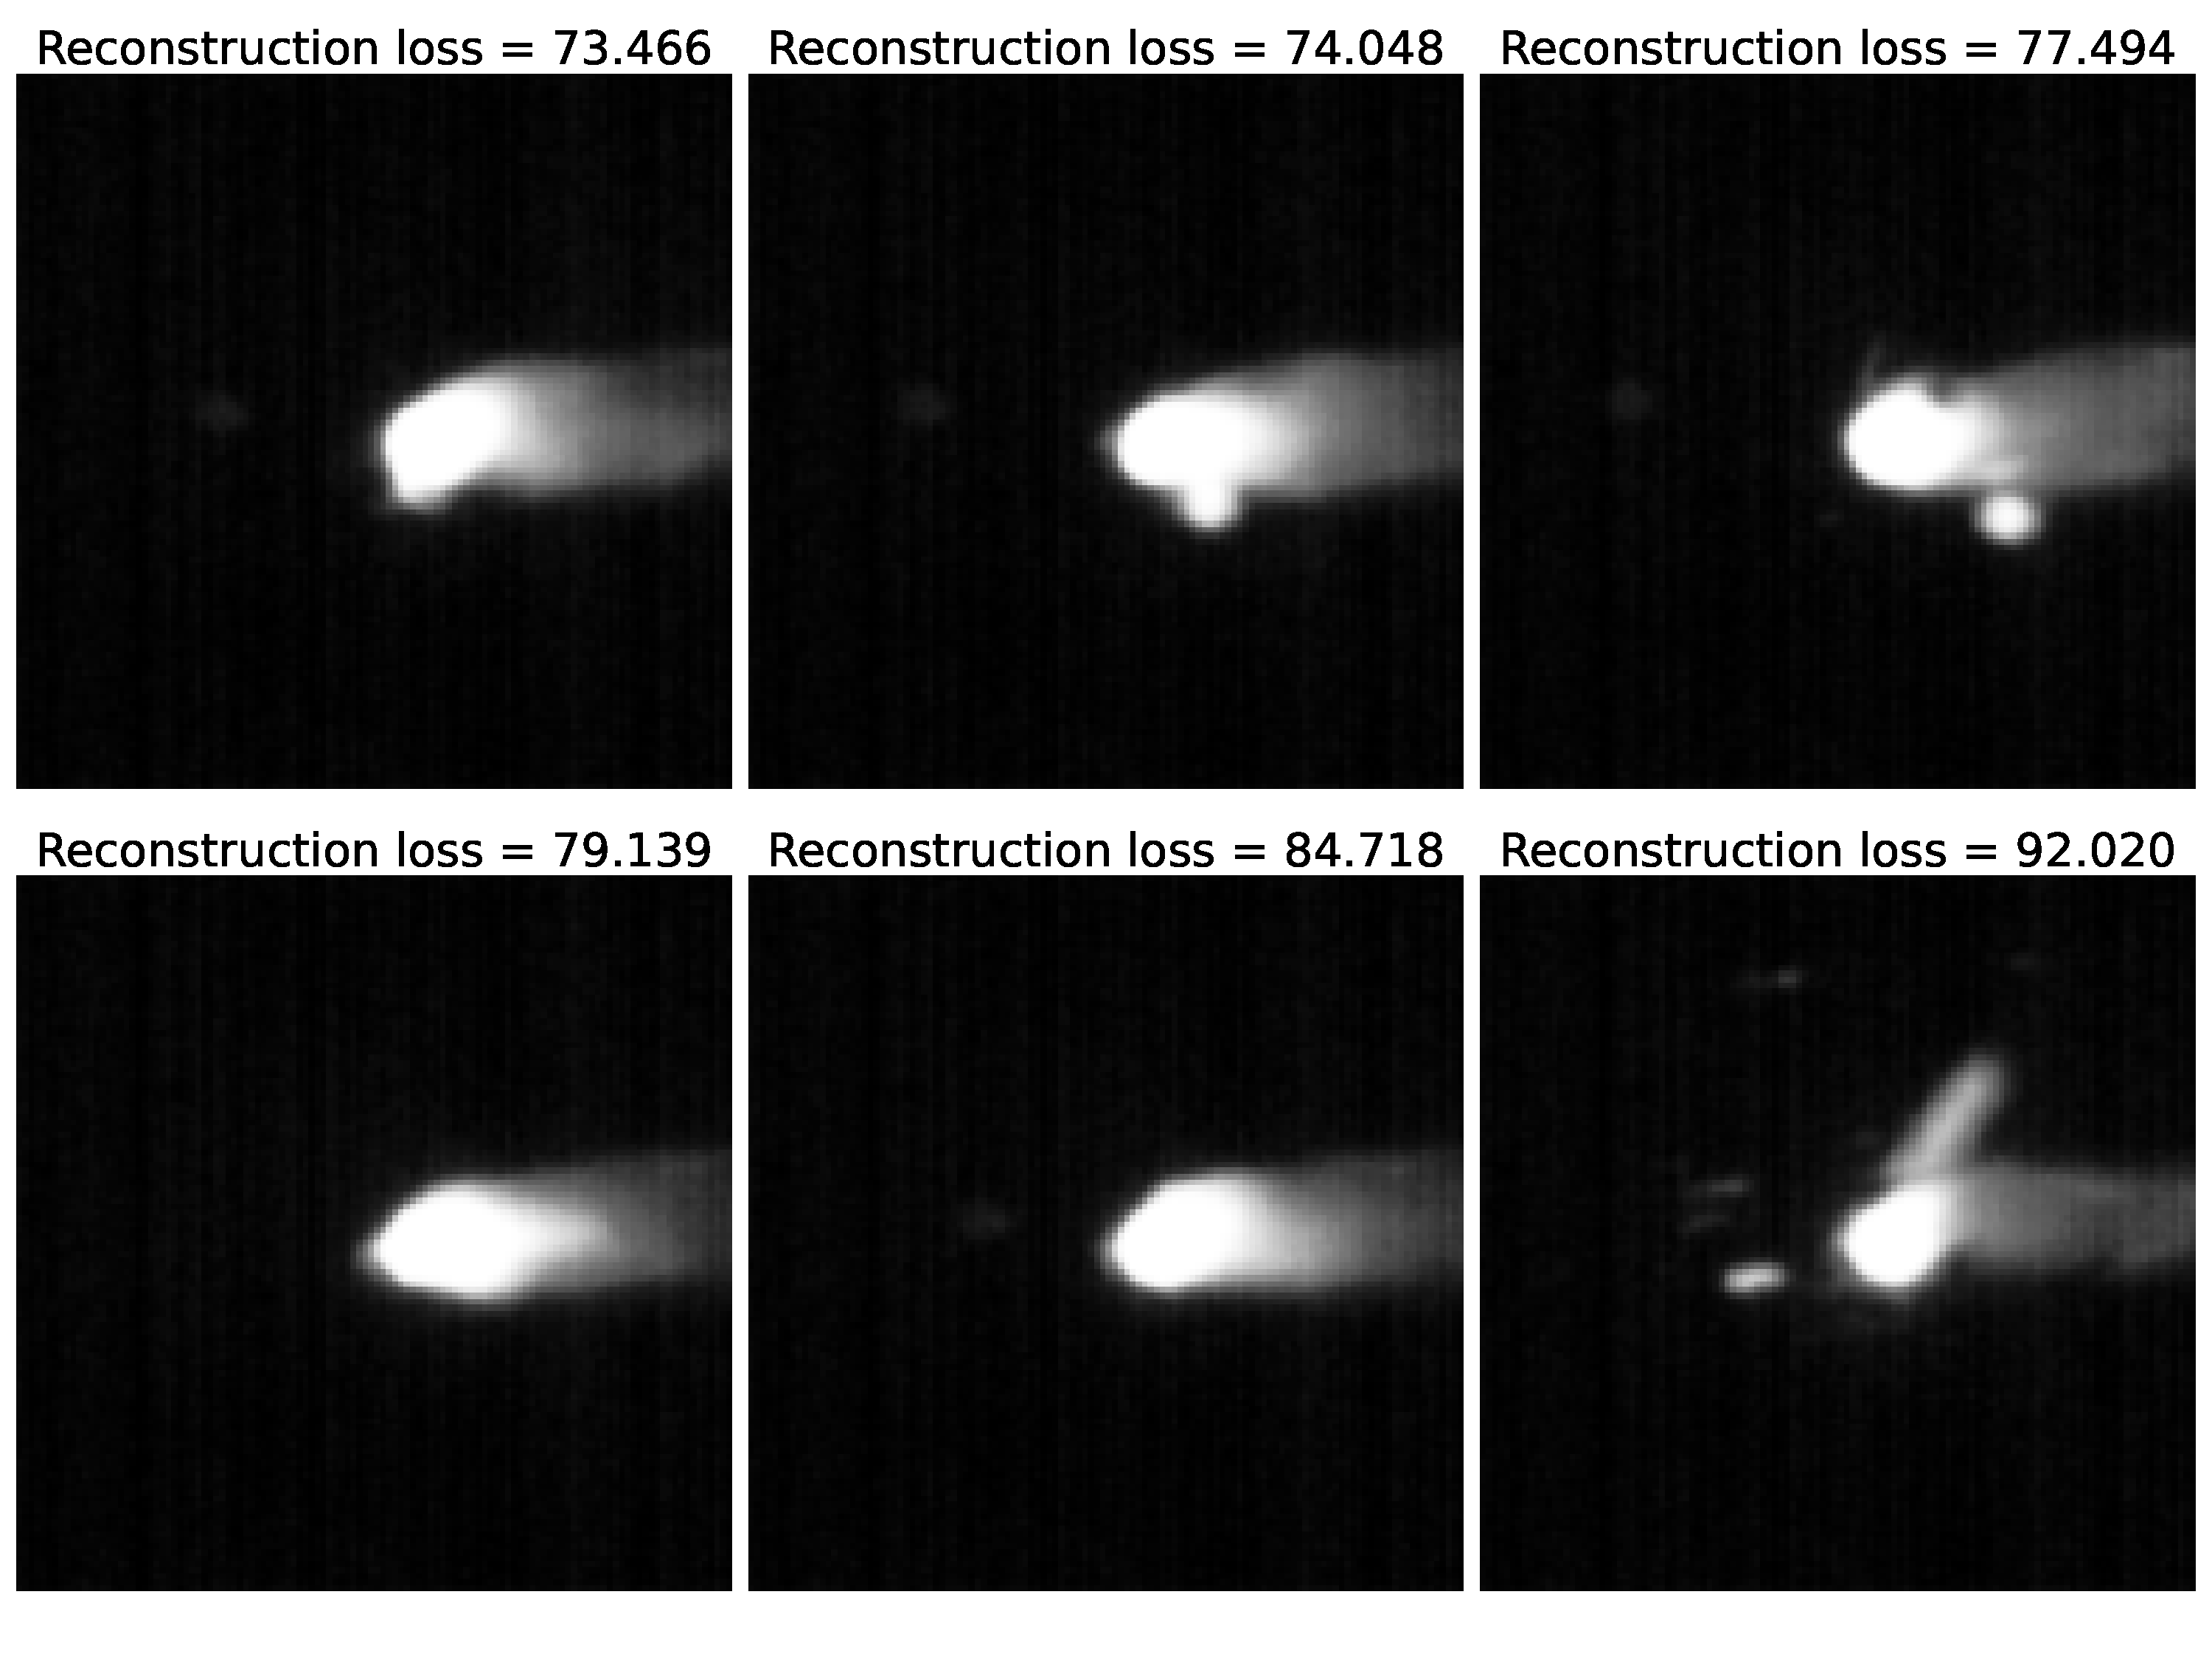
\includegraphics[scale=.15]{model_4_after_test_worst.pdf}
            \caption{Примеры худших по значению функционала ошибки восстановления кадров из валидационного набора \textbf{150A}.}\label{model_4_after_test_worst}
        \end{subfigure}
        \caption{Примеры найденных ConvLSTMAE, обученной на \textbf{210B} с размером окна 4, аномальных кадров. Над изображениями подписано значение функционала ошибки восстановления \eqref{mse}.}\label{lstm_worst_after}
    \end{figure}

    На полученном с помощью модели ConvLSTMAE наборе данных \textbf{210B}, была вновь обучена модель той же архитектуры. На Рис. \ref{lstm_worst_after} изображены найденные новой моделью аномальные кадры из наборов данных \textbf{210B} и \textbf{150A}. Можно отметить, что худшие по функционалу ошибки восстановления кадры из набора \textbf{210B} визуально не столь очевидно представляют опасность для процесса плавления, чем удалённые в результате очистки выборки \textbf{210A} (см. Рис. \ref{model_4_train_worst}), но всё так же являются результатами аномальных ситуаций (имеются в виду чёрные полости в ваннах расплава, свидетельствующие о мешающем лазеру наплавлении, а также сравнимые по площади с ванной всплески).

    На Рис. \ref{model_4_loss_distr_after} изображены распределения функционала ошибки восстановления итоговой модели на наборах данных \textbf{210A} и \textbf{150A}. Можно отметить, что в сравнении с Рис. \ref{model_4_loss_distr}, распределение ошибки на тестовой выборке стало более концентрированным, более <<прижатым>> к нулю, а значит и более похожим на распределение на обучающей выборке. Это свидетельствует о хорошей обобщающей способности получившегося алгоритма, а также о его приспособленности к применению к задаче поиска аномалий.


    \begin{figure}[]
        \centering
        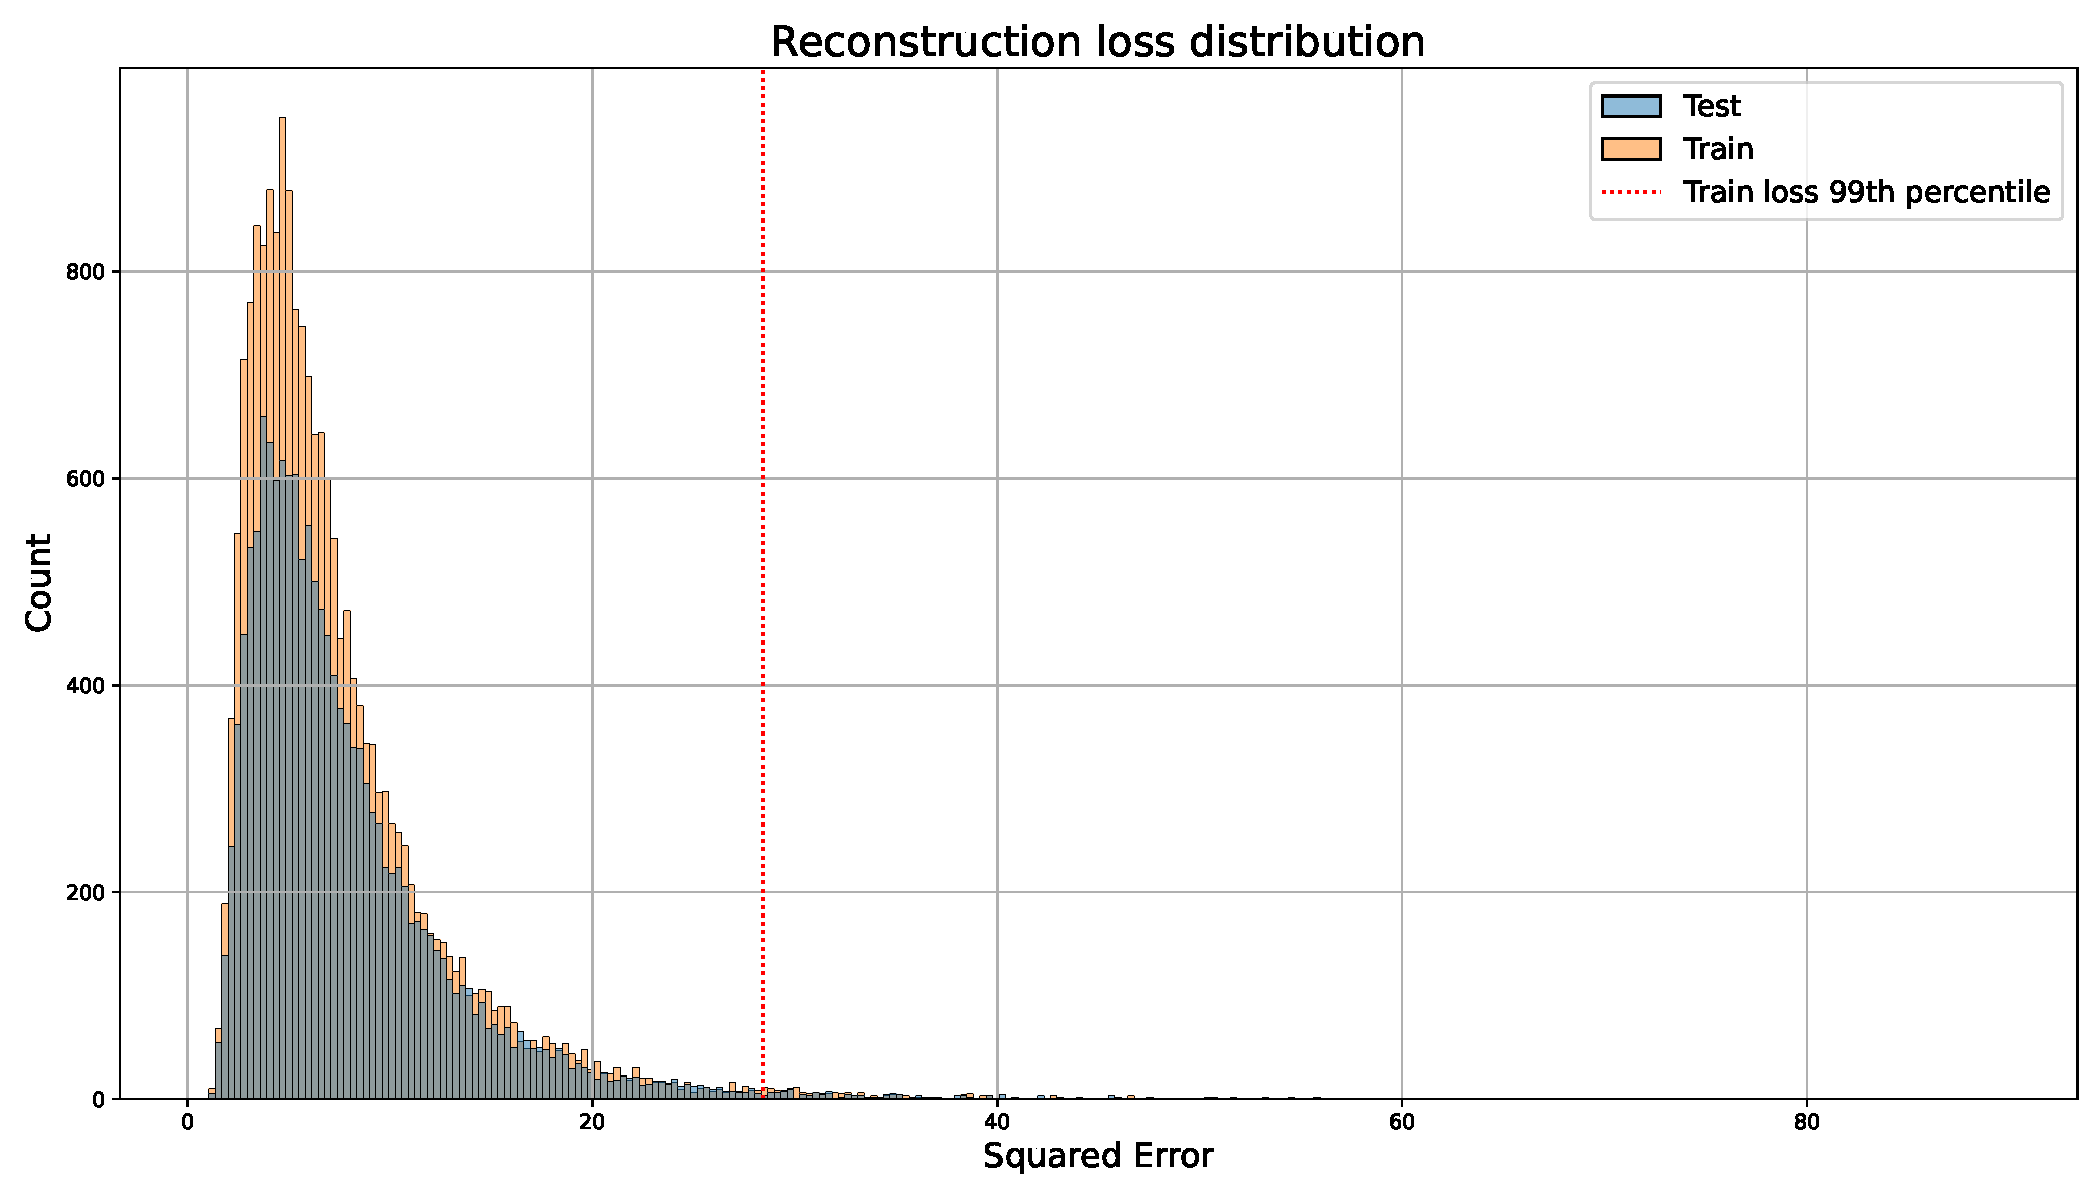
\includegraphics[scale=0.3]{model_4_loss_distr_after.pdf}
        \caption{Распределение значений функционала \eqref{mse} на обучающей и валидационной выборке для модели ConvLSTMAE, обученной на \textbf{210B} при значении размера окна равном 4.}
        \label{model_4_loss_distr_after}
    \end{figure}

    Помимо описанного выше исследования модели с размером окна, равным 4, были поставлены эксперименты по исследованию влияния иных значений данного гиперпараметра для модели ConvLSTMAE. В частности, были учтены значения в 2 и 6 кадров, составляющих последовательность, подающуюся на вход нейронной сети. Каждая из моделей была обучена на <<очищенном>> наборе данных \textbf{210B}. На Рис. \ref{model_2_loss_distr} и \ref{model_6_loss_distr} можно наблюдать распределения функционала ошибки восстановления, получаемые с помощью таких моделей, а распределения ошибки \eqref{mse} по координатной плоскости для всех методов отображены в Приложении \ref{app:distrs}. Сравнение всех рассматриваемых в работе моделей представлено в разделе \ref{comparison}.

    \begin{figure}[]
        \centering
            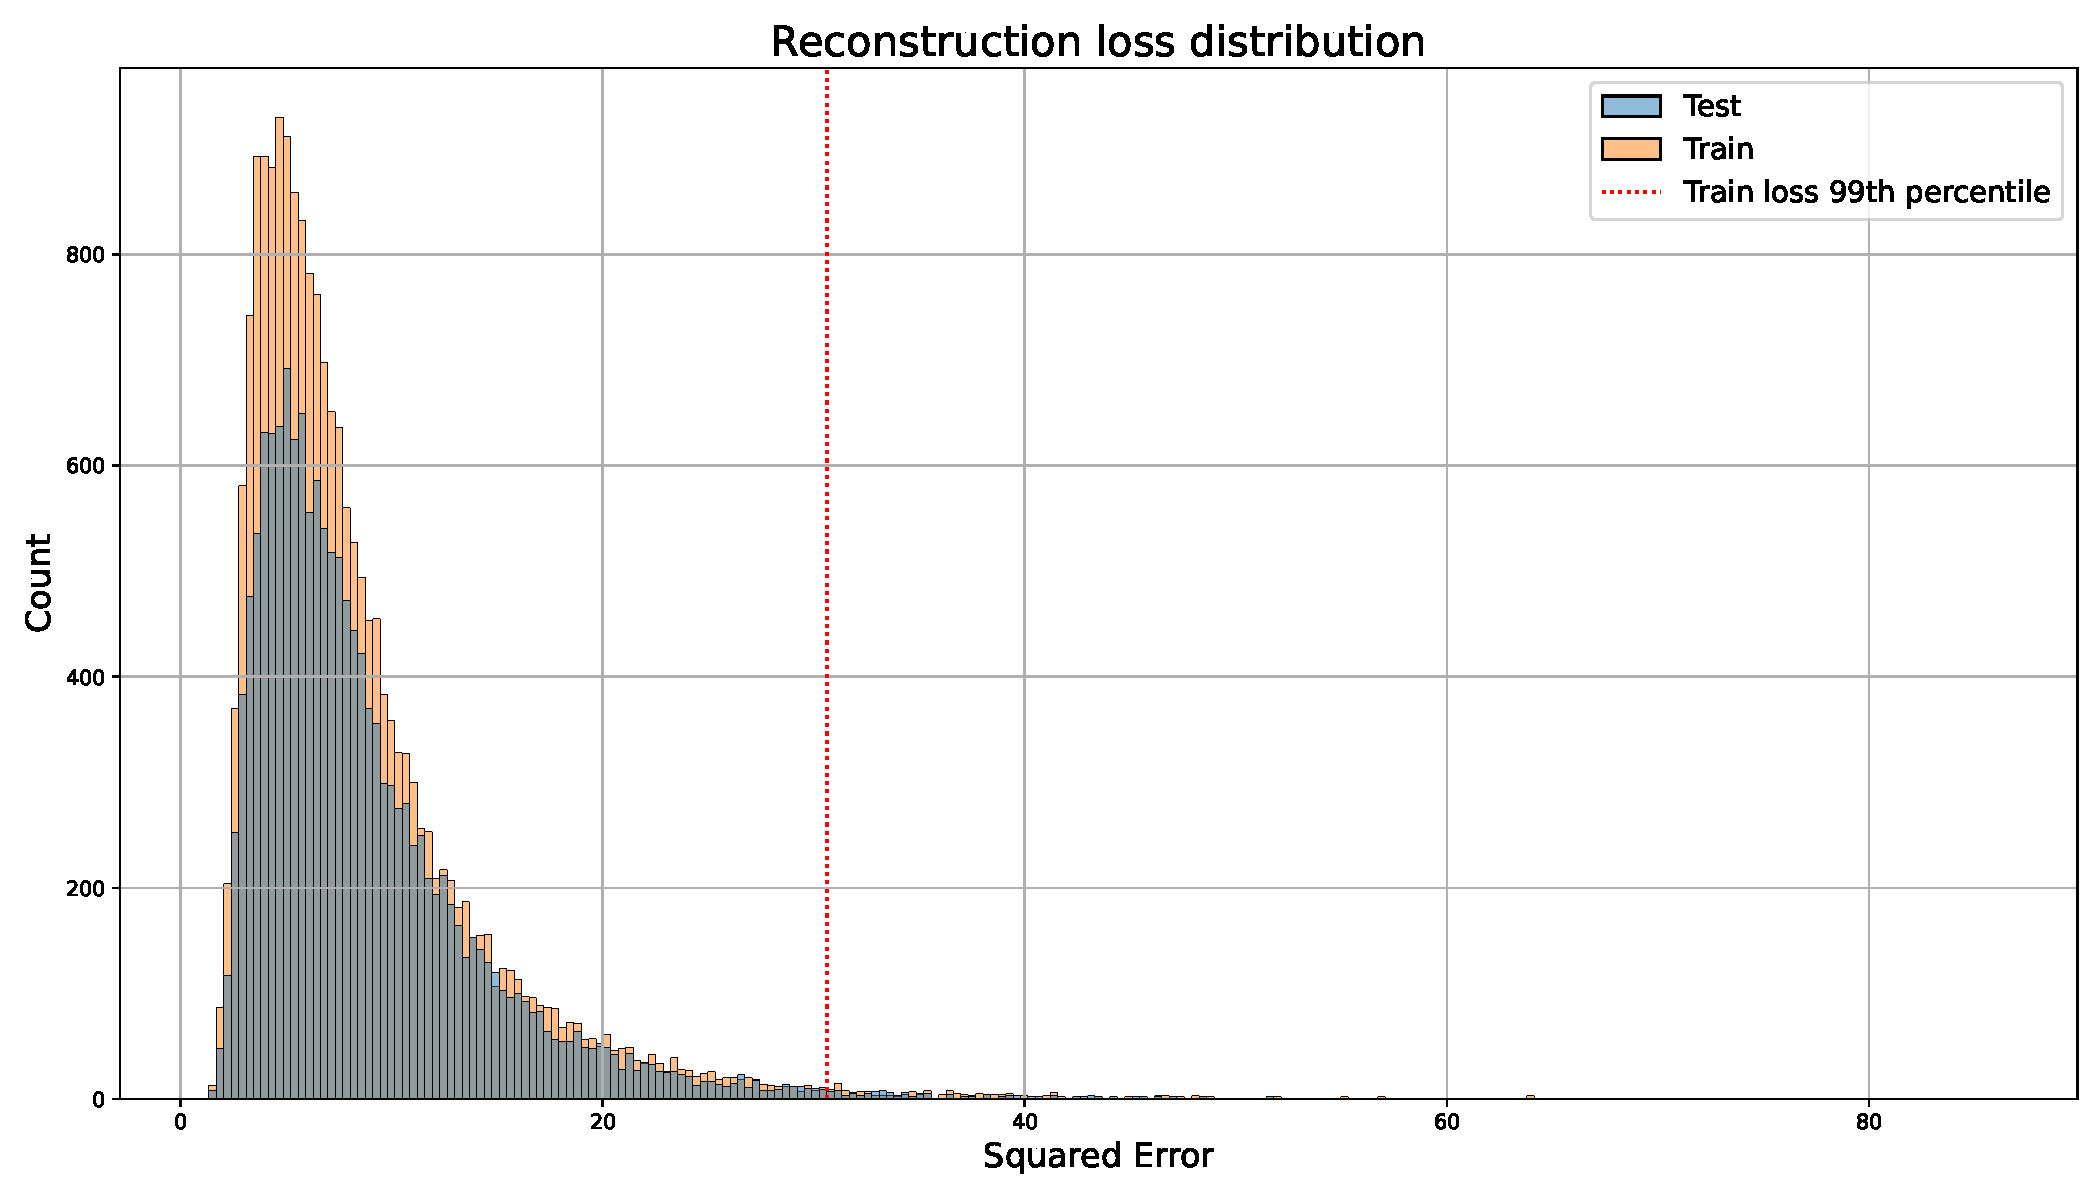
\includegraphics[scale=.3]{model_2_loss_distr.pdf}
            \caption{Распределение значений функционала \eqref{mse} на обучающей и валидационной выборке для модели ConvLSTMAE, обученной на \textbf{210B} при значении размера окна равном 2.}\label{model_2_loss_distr}
        \centering
    \end{figure}
    
    \begin{figure}[]
        \centering
            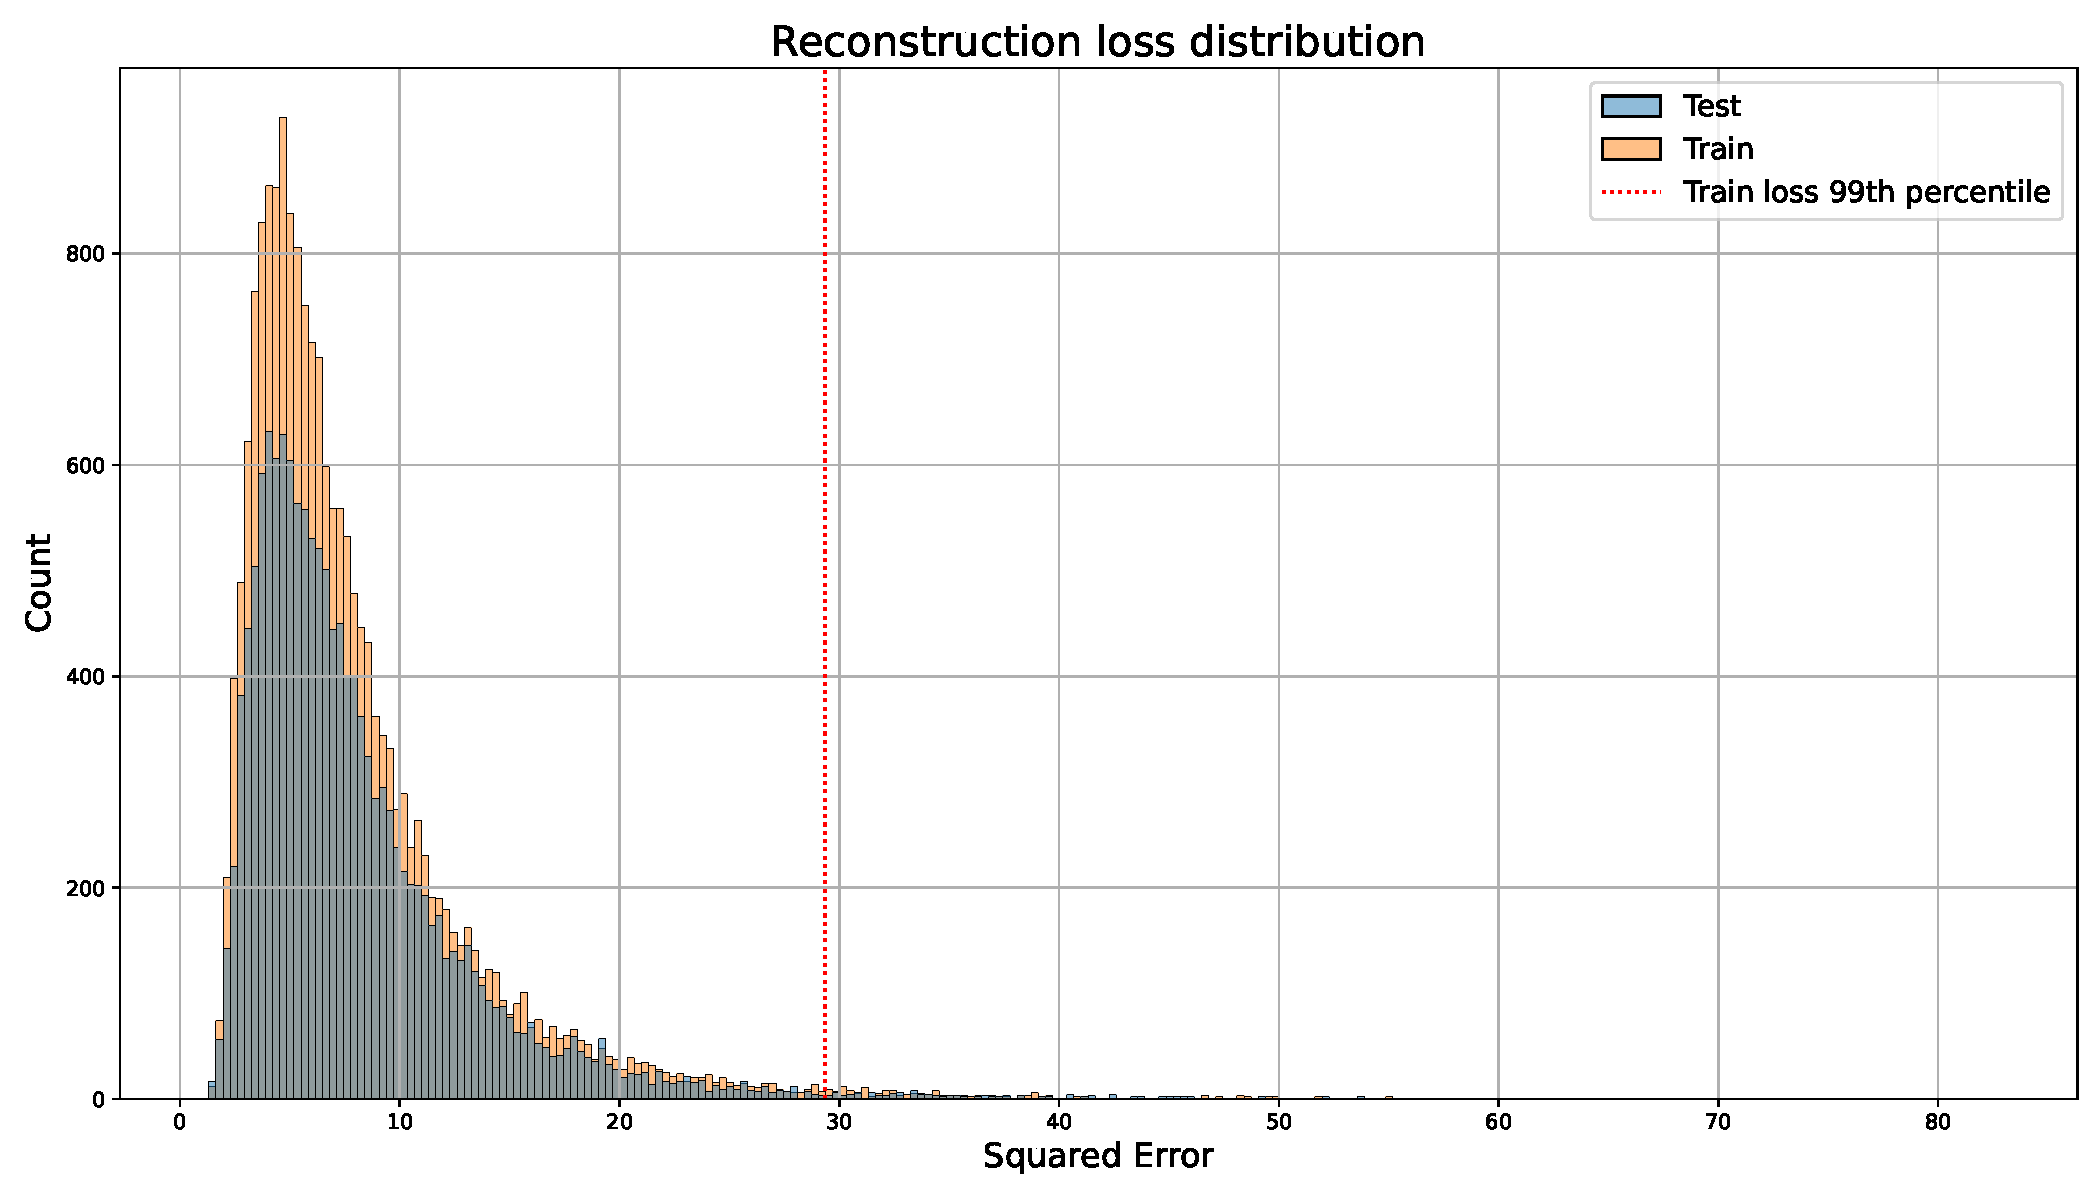
\includegraphics[scale=.3]{model_6_loss_distr.pdf}
            \caption{Распределение значений функционала \eqref{mse} на обучающей и валидационной выборке для модели ConvLSTMAE, обученной на \textbf{210B} при значении размера окна равном 6.}\label{model_6_loss_distr}
        \end{figure}



\bibliographystyle{unsrtnat}
\bibliography{references}


\newpage
\appendix
\addcontentsline{toc}{section}{Приложение}
\renewcommand{\thesubsection}{\Alph{subsection}}

\begin{subsection}{Архитектуры нейронных сетей \label{app:archs}}

    \begin{table}[H]
    \centering
    \small
    \begin{tabular}{@{}llccccc@{}}
    \toprule
    \multicolumn{1}{c}{} & \multicolumn{1}{c}{Слой} & \begin{tabular}[c]{@{}c@{}}Число каналов\\ (вход/выход)\end{tabular} & \begin{tabular}[c]{@{}c@{}}Размер\\ фильтра\end{tabular} & Шаг            & \begin{tabular}[c]{@{}c@{}}Доп.\\ действия\end{tabular}   & Активация \\ \midrule
    \multirow{9}{*}{Кодировщик}    & Conv3D                    & 1/64                                                        & $3 \times 3 \times 3$                                     & 1                 & -                                                               & ReLU       \\
                                & Conv3D                    & 64/64                                                       & $3 \times 3 \times 3$                                     & 1                 & \begin{tabular}[c]{@{}c@{}}Сохранить\\ активацию 1\end{tabular} & ReLU       \\
                                & MaxPool3D                 & 64/64                                                       & $1 \times 2 \times 2$                                     & $1 \times 2 \times 2$ & -                                                               & -          \\
                                & Conv3D                    & 64/128                                                      & $3 \times 3 \times 3$                                     & 1                 & -                                                               & ReLU       \\
                                & Conv3D                    & 128/128                                                     & $3 \times 3 \times 3$                                     & 1                 & \begin{tabular}[c]{@{}c@{}}Сохранить\\ активацию 2\end{tabular} & ReLU       \\
                                & MaxPool3D                 & 128/128                                                     & $1 \times 2 \times 2$                                     & $1 \times 2 \times 2$ & -                                                               & -          \\
                                & Conv3D                    & 128/256                                                     & $3 \times 3 \times 3$                                     & 1                 & -                                                               & ReLU       \\
                                & Conv3D                    & 256/256                                                     & $3 \times 3 \times 3$                                     & 1                 & -                                                               & ReLU       \\
                                & MaxPool3D                 & 256/256                                                     & $1 \times 2 \times 2$                                     & $1 \times 2 \times 2$ & -                                                               & -          \\ \midrule
    \multirow{8}{*}{Декодировщик}    & Interpolation             & 256/256                                                     & $1 \times 2 \times 2$                                     & -                 & -                                                               & -          \\
                                & Conv3D                    & 256/128                                                     & $3 \times 3 \times 3$                                     & 1                 & \begin{tabular}[c]{@{}c@{}}Прибавить\\ активацию 2\end{tabular} & -          \\
                                & Conv3D                    & 128/128                                                     & $3 \times 3 \times 3$                                     & 1                 & -                                                               & ReLU       \\
                                & Conv3D                    & 128/128                                                     & $3 \times 3 \times 3$                                     & 1                 & -                                                               & ReLU       \\
                                & Interpolation             & 128/128                                                     & $1 \times 2 \times 2$                                     & -                 & -                                                               & -          \\
                                & Conv3D                    & 128/64                                                      & $3 \times 3 \times 3$                                     & 1                 & \begin{tabular}[c]{@{}c@{}}Прибавить\\ активацию 1\end{tabular} & -          \\
                                & Conv3D                    & 64/64                                                       & $3 \times 3 \times 3$                                     & 1                 & -                                                               & ReLU       \\
                                & Conv3D                    & 64/64                                                       & $3 \times 3 \times 3$                                     & 1                 & -                                                               & ReLU       \\ \midrule
    \multirow{2}{*}{Выход}      & Conv3D                    & 64/1                                                        & $1 \times 1 \times 1$                                     & 1                 & -                                                               & Sigmoid    \\
                                & MaxPool3D                 & 1/1                                                         & $4 \times 1 \times 1$                                     & 1                 & -                                                               & -          \\ \bottomrule
    \end{tabular}
    \caption{Архитектура нейронной сети UNET3d. Отказ от конкатенации активаций в пользу сложения обусловлен отсутствием потерь в качестве и ускорением работы нейронной сети.}
    \label{tab:unet_arch}
    \end{table}


    \begin{table}[H]
    \centering
    \scriptsize
    \begin{tabular}{@{}llccccc@{}}
    \toprule
    \multicolumn{1}{c}{}     & \multicolumn{1}{c}{Слой}         & \begin{tabular}[c]{@{}c@{}}Число каналов\\ (вход/выход)\end{tabular} & \begin{tabular}[c]{@{}c@{}}Размер\\ фильтра\end{tabular} & Страйд & \begin{tabular}[c]{@{}c@{}}Доп.\\ действия\end{tabular}            & Активация \\ \midrule
    \multirow{4}{*}{Кодировщик} & Conv2D\_TimeDistributed          & 1/128                                                                & $5 \times 5$                                             & 2      & -                                                                  & ReLU      \\
                             & BatchNorm2D\_TimeDistributed     & 128/128                                                              & -                                                        & -      & -                                                                  & -         \\
                             & Conv2D\_TimeDistributed          & 128/64                                                               & $5 \times 5$                                             & 2      & -                                                                  & ReLU      \\
                             & BatchNorm2D\_TimeDistributed     & 64/64                                                                & -                                                        & -      & -                                                                  & -         \\ \midrule
    \multirow{3}{*}{LSTM}   & ConvLSTM                         & 64/32                                                                & $5 \times 5$                                             & 1      & \begin{tabular}[c]{@{}c@{}}Dropout, 0.1\\ LayerNorm\end{tabular} & ReLU      \\
                             & ConvLSTM                         & 32/64                                                                & $5 \times 5$                                             & 1      & \begin{tabular}[c]{@{}c@{}}Dropout, 0.1\\ LayerNorm\end{tabular} & ReLU      \\
                             & BatchNorm2D\_TimeDistributed     & 64/64                                                                & -                                                        & -      & -                                                                  & -         \\ \midrule
    \multirow{5}{*}{Декодировщик} & Conv2DTranspose\_TimeDistributed & 64/64                                                                & $5 \times 5$                                             & 2      & -                                                                  & ReLU      \\
                             & BatchNorm2D\_TimeDistributed     & 64/64                                                                & -                                                        & -      & -                                                                  & -         \\
                             & Conv2DTranspose\_TimeDistributed & 64/128                                                               & $5 \times 5$                                             & 2      & -                                                                  & ReLU      \\
                             & BatchNorm2D\_TimeDistributed     & 128/128                                                              & -                                                        & -      & -                                                                  & -         \\
                             & Conv2DTranspose\_TimeDistributed & 128/1                                                                & $5 \times 5$                                             & 2      & -                                                                  & Sigmoid   \\ \bottomrule
    \end{tabular}
    \caption{Архитектура нейронной сети ConvLSTMAE. Под использованием дропаута понимается применение этого механизма согласно статье Гала и Гарамани~\cite{gal2016theoretically}. LayerNorm применяется к изображению на каждом рекуррентном шаге ConvLSTM.}
    \label{tab:lstm_arch}
    \end{table}

\end{subsection}

\newpage

\begin{subsection}{Распределения функционала ошибки восстановления по координатам \label{app:distrs}}

    \begin{figure}[H]
        \centering
        \begin{subfigure}{.47\textwidth}
            \centering
            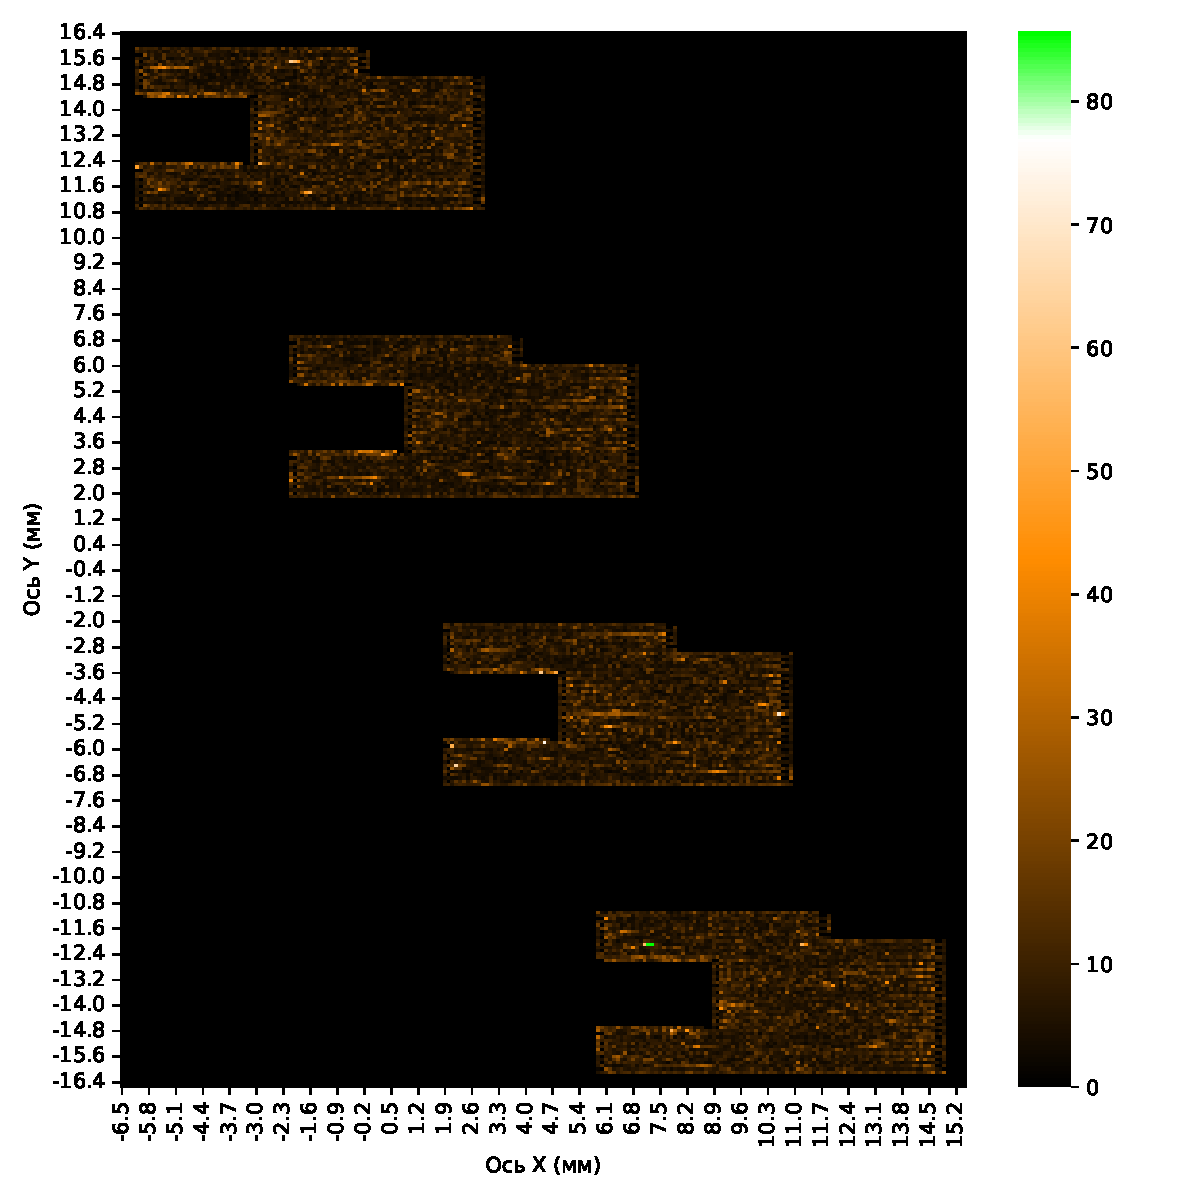
\includegraphics[scale=.3]{lstm_2_window_xy_train.pdf}
            \caption{Среднее по координате значение функционала ошибки восстановления для тренировочного набора \textbf{210A}.}\label{lstm_2_window_xy_train}
        \end{subfigure}
        \hfill
        \begin{subfigure}{.47\textwidth}
            \centering
            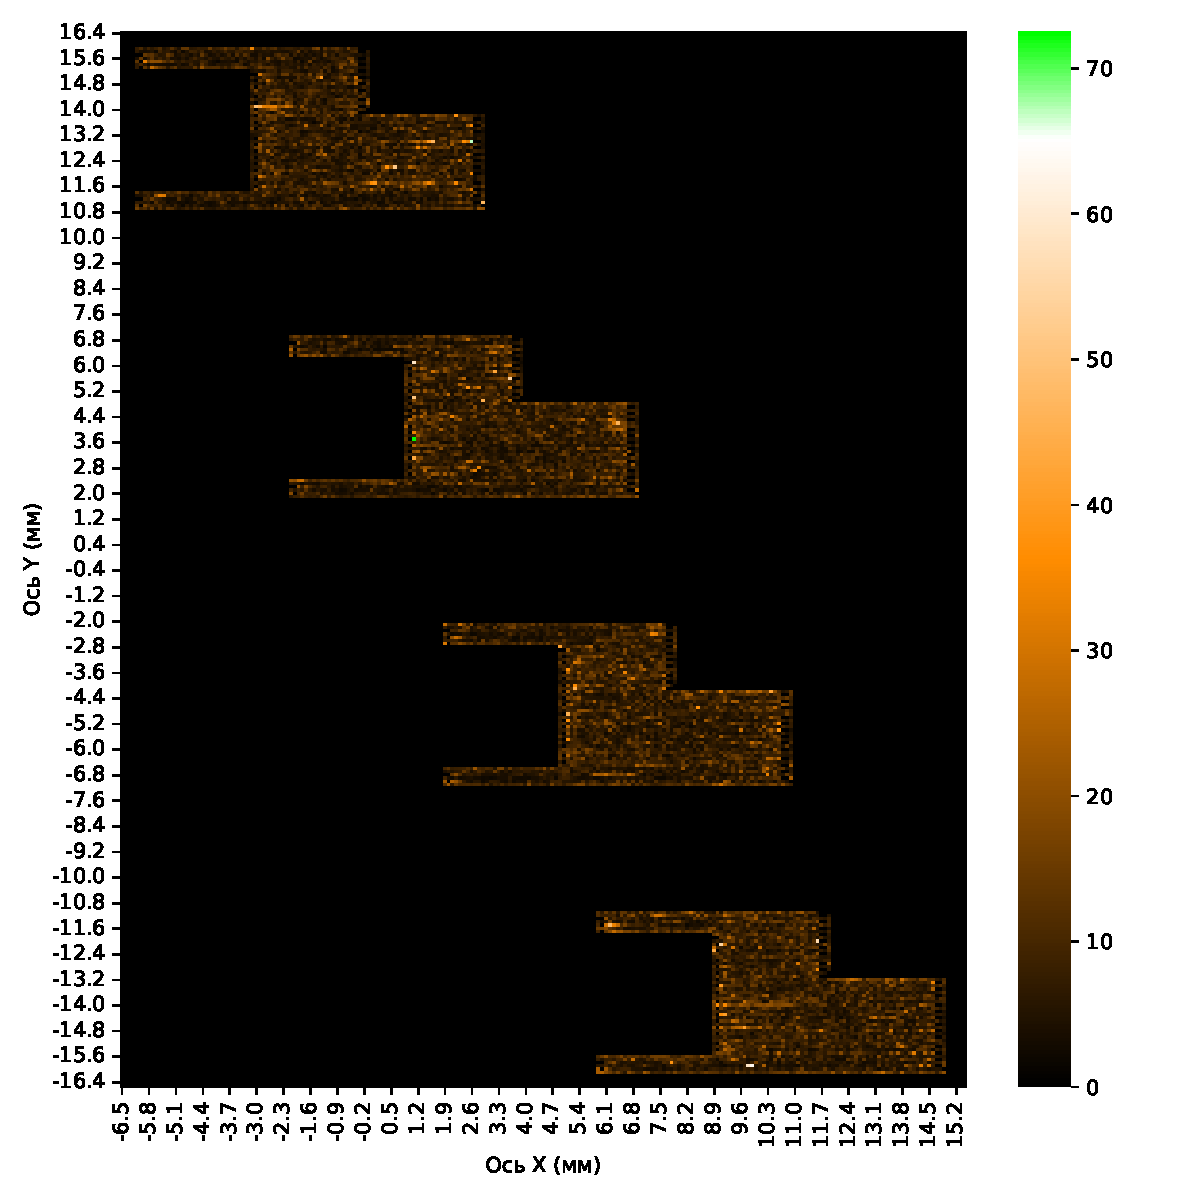
\includegraphics[scale=.3]{lstm_2_window_xy_test.pdf}
            \caption{Среднее по координате значение функционала ошибки восстановления для валидационного набора \textbf{150A}.}\label{lstm_2_window_xy_test}
        \end{subfigure}
        \caption{Распределение функционала \eqref{mse} по координате для модели ConvLSTMAE, обученной на \textbf{210B} с размером окна 2.}\label{lstm_xy_2}
    \end{figure}

    \begin{figure}[H]
        \centering
        \begin{subfigure}{.47\textwidth}
            \centering
            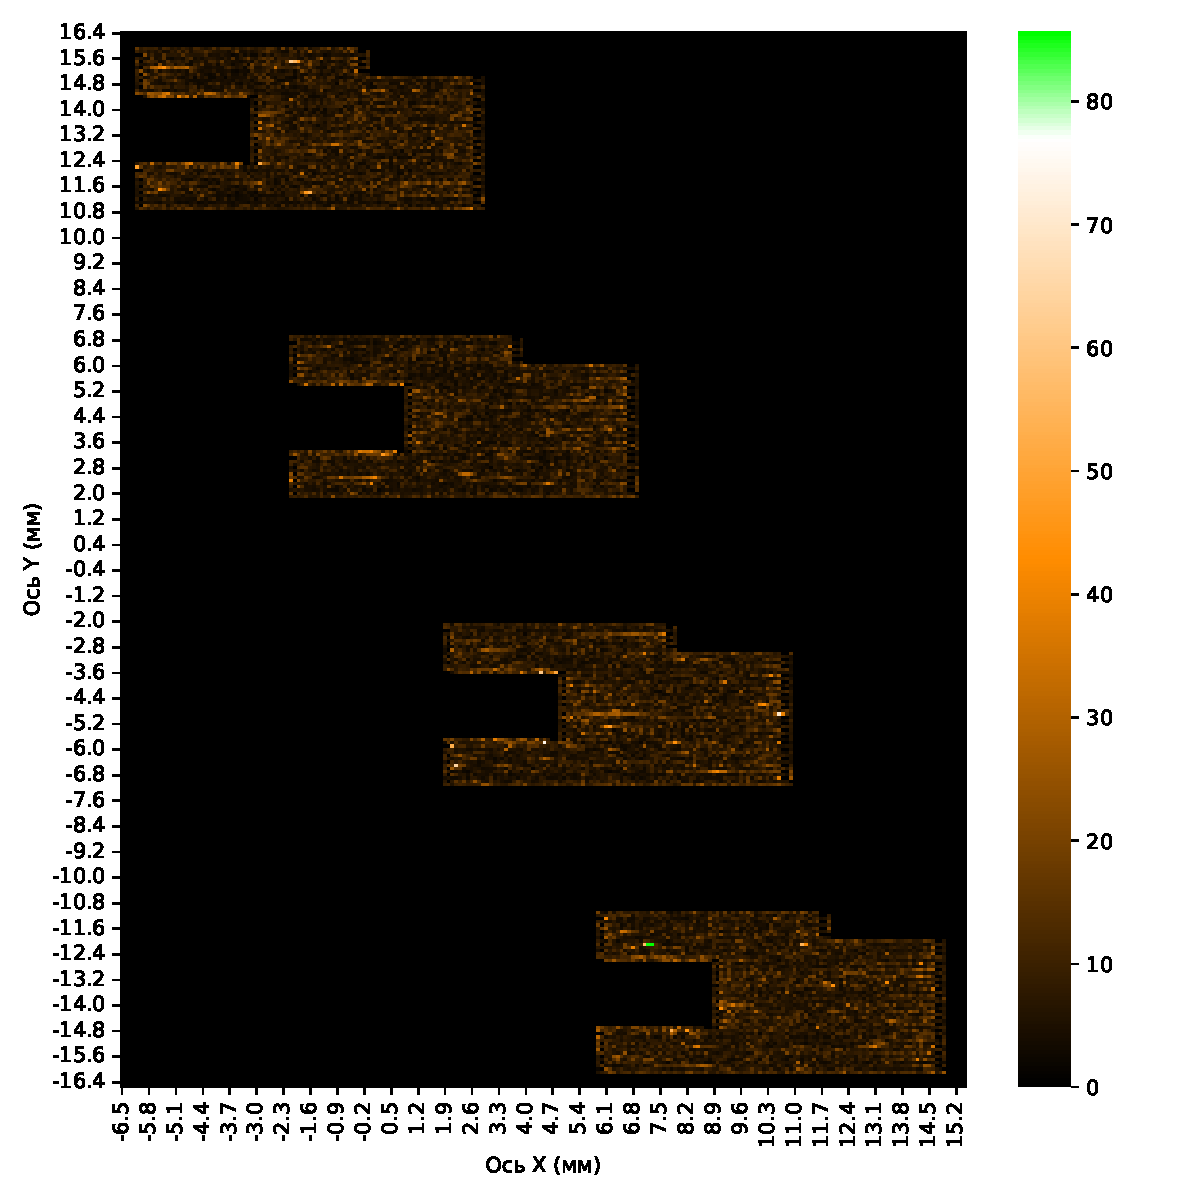
\includegraphics[scale=.3]{lstm_2_window_xy_train.pdf}
            \caption{Среднее по координате значение функционала ошибки восстановления для тренировочного набора \textbf{210A}.}\label{lstm_2_window_xy_train}
        \end{subfigure}
        \hfill
        \begin{subfigure}{.47\textwidth}
            \centering
            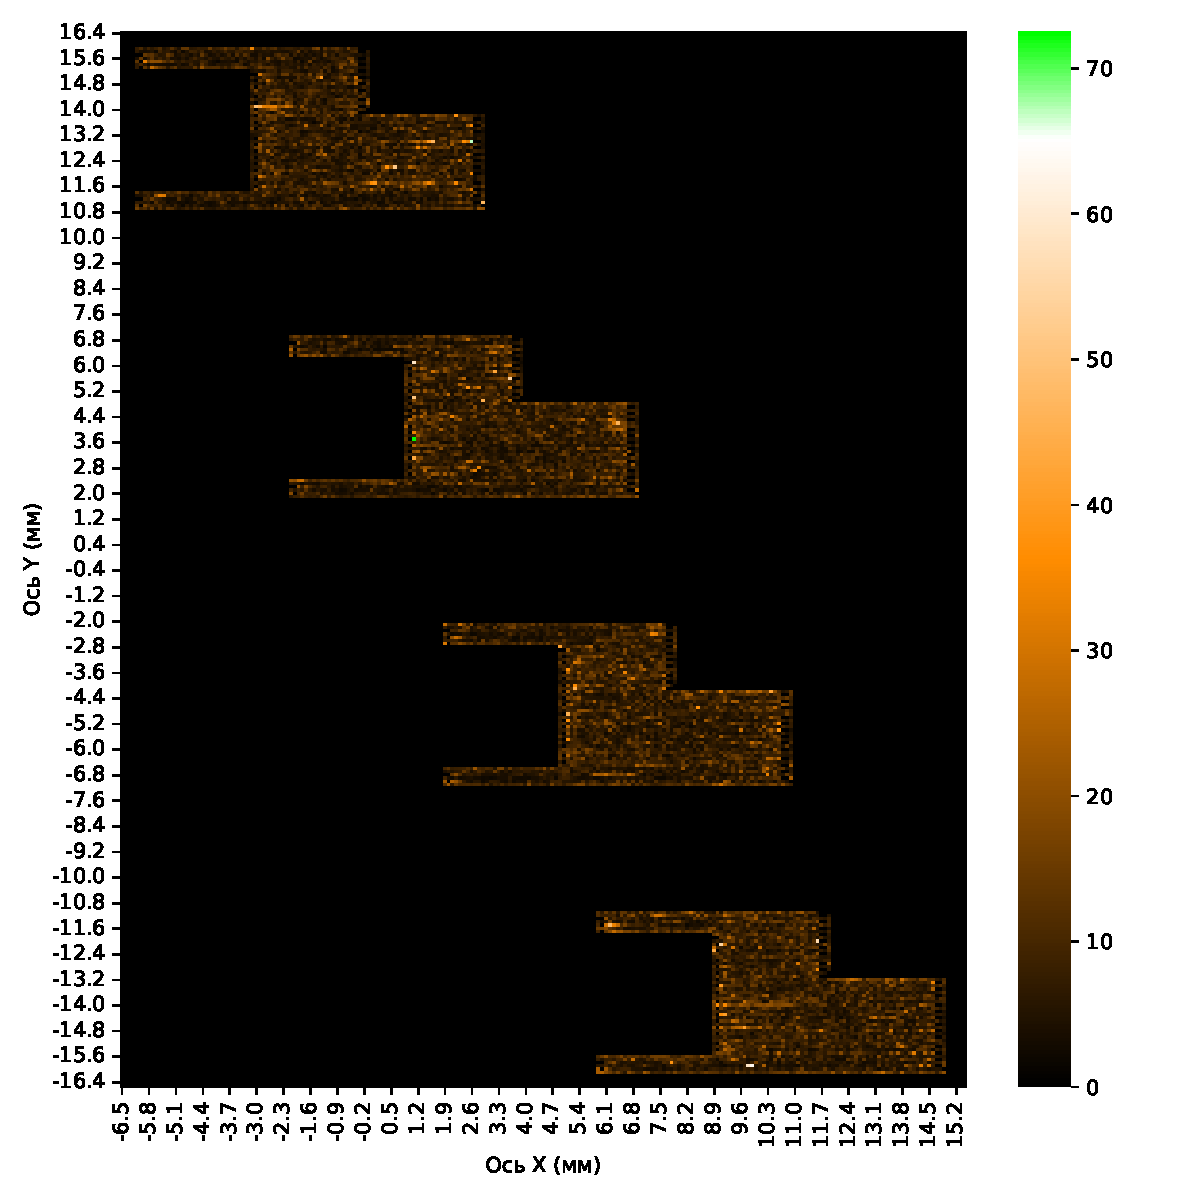
\includegraphics[scale=.3]{lstm_2_window_xy_test.pdf}
            \caption{Среднее по координате значение функционала ошибки восстановления для валидационного набора \textbf{150A}.}\label{lstm_2_window_xy_train}
        \end{subfigure}
        \caption{Распределение функционала \eqref{mse} по координате для модели ConvLSTMAE, обученной на \textbf{210B} с размером окна 6.}\label{lstm_xy_6}
    \end{figure}
\end{subsection}

\end{document}